\chapter{Implementación}
\label{chap:implementation}

En este capítulo se detallará la implementación técnica del proyecto.

\section{Arquitectura del proyecto}

La unidad de construcción mínima en Godot es el \textbf{nodo}. Cada nodo puede asignarse como hijo de otro nodo, y puede a su vez ser el padre de otros, formando así una estructura de árbol. Los nodos pueden contener un estado, una lógica que actualiza su estado a lo largo del tiempo, y una representación visual en la ejecución del juego. Es un elemento versátil que puede cumplir cualquier funcionalidad dentro de la arquitectura de un proyecto. Godot cuenta con tipos básicos de nodos, pero el desarrollador puede definir los suyos propios.

Una estructura de árbol de nodos se puede agrupar en lo que se denomina \textbf{escena}. Las escenas tienen un nodo raíz, y otros nodos que hacen de hijos, nietos, etc de esa raíz. Para entender mejor la filosofía de diseño de Godot, estos son algunos ejemplos de unidades lógicas que se pueden construir agrupando nodos en escenas:

\begin{itemize}
    \item Personaje del jugador: La escena tendría como raíz un nodo tipo CharacterBody2D (ideado para construir personajes que se mueven). Como hijos tendría un nodo CollisionShape2D para detectar colisiones, un Sprite2D para dibujar el personaje en pantalla y un script asociado a la raíz que implementa su estado y lógica.
    \item Menu de inicio: La escena sería tipo Node2D. Tendría como hijos un nodo Label para escribir el nombre del juego, y 3 nodos Button para representar los las opciones del menú: Jugar, Ajustes y Salir. El nodo raíz tendría un script asociado para implementar la lógica de los botones.
    \item Cinemática: La escena representaría una animación no interactiva dentro del motor del juego. Su nodo raíz sería del tipo Node2D. Contendría nodos para todos los elementos que participen en la escena (personajes, terreno, sonido, música) y un AnimationPlayer para animar todos estos elementos.
\end{itemize}

Las escenas son equivalentes a un nodo: empaquetan una funcionalidad y la ponen a disposición de otros nodos, pudiendo instanciarse una escena en múltiples lugares. Una escena puede tener como hijo a un nodo u otra escena. El resultado es que, en ejecución y en arquitectura, los proyectos de Godot forman un gran árbol de nodos y escenas. A este árbol se le llama \textit{scene tree}, o árbol de escenas. En la figura \ref{fig:scene-tree} se puede observar un ejemplo de este durante la ejecución del juego.

\begin{figure}[h]
    \centering
    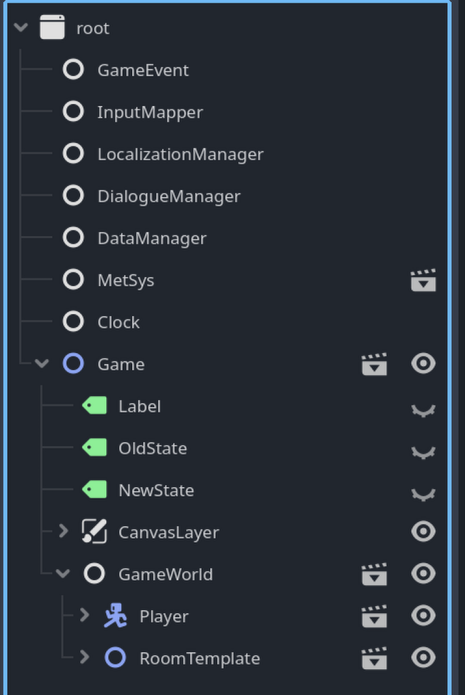
\includegraphics[scale=0.7]{img/scene_tree.png}
    \caption[Scene Tree de ejecución de Godot]{Scene Tree en un instante de ejecución del proyecto.}
    \label{fig:scene-tree}
\end{figure}

Otro elemento fundamental de Godot son las \textbf{señales}. Estas son un mecanismo de delegación que permite a un nodo reaccionar a un evento que ocurre en otro nodo. Por ejemplo, la escena Jugador podría declarar una señal que se emite cuando este recibe daño. La escena InterfazDeJuego, por otro lado, conectaría una función a la señal de Jugador que se encargaría de actualizar la salud restante en la interfaz. Esto permite la comunicación entre nodos que son lejanos entre si en el scene tree, reduciendo también el acoplamiento del proyecto.

A la hora de diseñar arquitecturas en Godot, es indispensable pensarla en términos de nodos y escenas. Por eso mismo, en la figura \ref{fig:proyect-architecture} se describe la arquitectura del proyecto como un árbol de escenas y no como, por ejemplo, un diagrama de clases. En esta cada nodo es una escena del proyecto. A lo largo de este capíutlo se desarrollarán en detalle cada una de las escenas. Por ahora y para adquirir una visión general del proyecto, se destacan:

\begin{itemize}
    \item \textbf{Game}: La lógica de esta escena sigue un patrón de máquina de estados. Se encarga de instanciar y eliminar las distintas pantallas que conforman el juego (menú principal, menú de pausa, pantalla de juego, pantalla de game over, etc).
    \item \textbf{GameWorld}: Es la escena que contiene y gestiona el mundo del videojuego: todos los niveles y elementos que lo componen como los personajes.
    \item \textbf{PlayerCharacter}: Es de los nodos más complejos del proyecto. Se encarga de gestionar el personaje del jugador: desde sus visuales, animaciones, lógica, controles, sonido, etc.
\end{itemize}

Los \textbf{Autoloads} son los nodos que se muestran arriba a la izquierda de la figura \ref{fig:proyect-architecture}. Estos son similares a un patrón Singleton: son cargados al inicio de la ejecución y existen como entidad única de su tipo. Son accesibles de forma global y normalmente su labor es la gestión de sistemas y prestación de servicios que pueden ser solicitados desde cualquier lugar del árbol de escena. Se desarrollarán más adelante en este capítulo.

\begin{figure}[h]
    \centering
    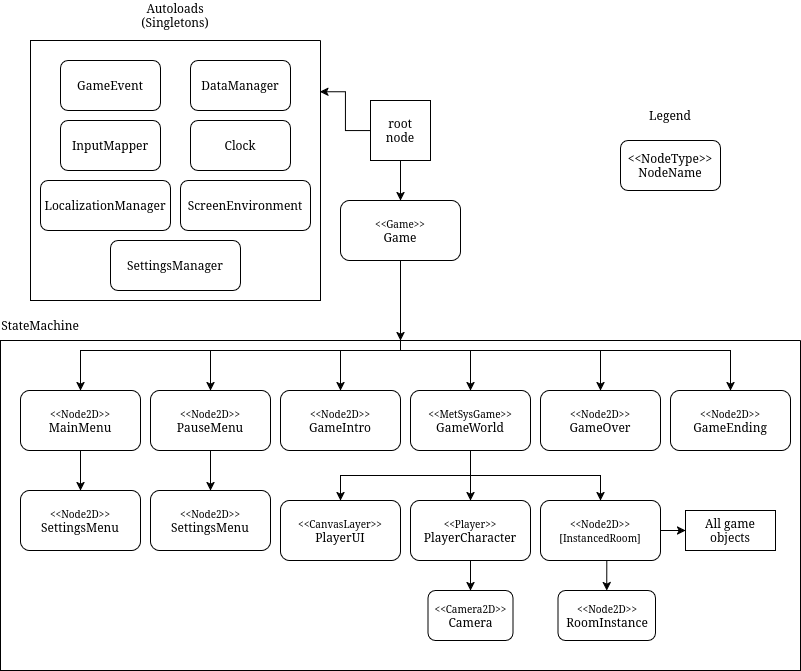
\includegraphics[scale=0.5]{img/proyect_architecture.drawio.png}
    \caption[Arquitectura general del proyecto]{Arquitectura general del proyecto}
    \label{fig:proyect-architecture}
\end{figure}

\subsection{Ciclo de vida de un nodo}

% Escribir sobre ready, process, delta time, etc

Cuando un nodo o escena es añadido durante la ejecución, se procesa su función \textit{\_ready()}. Esta puede ser sobreescrita desde el script de cualquier nodo para que realice las preparaciones que sean pertinentes como por ejemplo iniciar la animación de un personaje. Una vez termina de procesarse \textit{\_ready()}, se llama automáticamente a la misma función para todos los nodos hijos. Así sucesivamente, recorriendo todo el scene tree.

Para actualizar el estado del nodo en tiempo real se emplea la función \textit{\_process(delta: float)}. Esta es ejecutada para cada nodo una vez por fotograma y previamente al renderizado de la pantalla. El parámetro \textit{delta} corresponde al \textbf{tiempo delta}. Representa el tiempo transcurrido desde el último fotograma renderizado y se usa para mantener las velocidades consistentes entre distintos dispositivos. Si un personaje avanzara 100 píxeles de distancia en cada fotograma se movería más rápido en equipos más potentes, ya que son capaces de renderizar más fotogramas por segundo. De la misma forma, se movería más lento si aumentara el tiempo entre fotogramas debido a un pico de estrés. Es por eso que todas las velocidades del juego se multiplican por el tiempo delta, para ser consistentes.

El método \textit{\_process\_physics(delta: float)} es similar al anterior, pero es ejecutado una vez por cada \textit{tick} del motor de físicas, en lugar de cada fotograma. Por defecto Godot ejecuta los métodos de simulación de físicas 60 veces (ticks) por segundo, por lo que el código relativo a las físicas debe ir aquí en lugar de en \textit{\_process(delta: float)} para evitar comportamientos indeseados.

Para registrar los inputs que genera el jugador, se pueden consumir desde la función \textit{\_input(event: InputEvent)} o bien usando el singleton \textit{Input} desde \textit{\_process(delta: float)}.

Por último, la escena es eliminada del árbol y destruida cuando se llama a \textit{free()} o \textit{queue\_free()}. Esto provoca que se destruyan también sus hijos.

\subsection{Nodo Game}

El nodo Game es la raíz del proyecto. Su función es gestionar el ciclo de vida del juego, instanciando como hijos y liberando nodos para que el usuario pueda navegar por las distintas pantallas del programa. En la figura \ref{fig:game-state-diagram} se tiene el diagrama de estados para el nodo. Los estados corresponden a las siguientes pantallas de juego:

\begin{figure}[h]
    \centering
    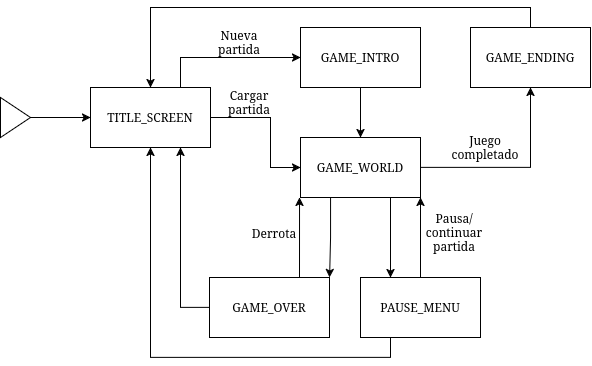
\includegraphics[scale=0.5]{img/GameLyfecycle.drawio.png}
    \caption[Diagrama de estados de nodo Game]{Diagrama de máquina de estados del nodo Game, correspondiente al ciclo de vida del juego}
    \label{fig:game-state-diagram}
\end{figure}

\begin{itemize}
    \item \textbf{TITLE\_SCREEN}: Corresponde a la pantalla de título del juego. Desde aquí se puede iniciar o cargar una partida. También se tiene acceso al menú de ajustes del juego y la opción de cerrar el programa.
    \item \textbf{GAME\_INTRO}: Esta escena contiene una animación que se reproduce cuando se inicia una nueva partida para dar contexto a la historia del juego.
    \item \textbf{GAME\_WORLD}: Este es el nodo donde se desarrolla toda la acción del juego. En este se instancian el jugador y el mundo del juego, con todos los elementos que lo conforman.
    \item \textbf{GAME\_OVER}: Cuando el jugador es derrotado se llega a esta pantalla, donde puede elegir si volver a intentarlo o regresar al menú.
    \item \textbf{PAUSE\_MENU}: El menú de pausa del juego. El nodo Game es responsable también de pausar (es decir, congelar) todo el árbol de escenas que cuelga de él cuando es necesario.
    \item \textbf{GAME\_ENDING}: Similar a GAME\_INTRO, esta escena contiene una animación con el final del juego. Tras acabar, se vuelve al menú principal.
\end{itemize}

La máquina de estados se realizó en el propio script del nodo, lo que suponía una implementación liviana apropiada para una máquina con una complejidad baja. El script define los estados posibles y hace que el nodo recuerde su estado actual, ya que está cargado en memoria en todo momento. Tiene funciones en las que se define qué debe ejecutar al entrar a un estado y al salir de otro. También define qué transiciones de estado están permitidas, y lanza errores cuando se intenta llevar a cabo una que no lo está. Cualquier nodo del scene tree puede solicitar un cambio de estado a través de una señal del nodo \textbf{GameEvent} (explicado a continuación). Game escucha las señales de GameEvent y lleva a cabo los cambios de estado pertinentes.

\subsection{Autoloads y GameEvent}

Los \textbf{Autoloads} son nodos que permiten la implementación del patrón singleton en Godot. Estos se cargan al inicio de la ejecución de un programa y permanecen siempre en memoria como hijos del nodo raíz. Godot guarda una referencia a ellos de tal forma que son accesibles desde cualquier nodo del scene tree aunque no estén directamente relacionados. En el proyecto se usan varios autoloads para distintas labores como se refleja en la figura \ref{fig:proyect-architecture}, siendo \textbf{GameEvent} la más relevante para la arquitectura del mismo.

GameEvent implementa un patrón de bus de eventos para el proyecto. El patrón de bus de evento consiste en deinir un cauce de comunicación entre distintos actores. Los nodos pueden enviar señales a través de ese cauce. El resto de nodos lo reciben y deciden si quieren consumirlo. En este proyecto, ese cauce es el autoload GameEvent haciendo uso de las señales de Godot, y los actores son cualquier nodo que exista en el proyecto.

GameEvent define y expone un catálogo de señales a las que otros nodos pueden conectarse o emitir. Esto permite, por ejemplo, que cuando el jugador es derrotado, el nodo Player emita la señal \textit{\_on\_game\_over}. El nodo Game recibe esta señal y cambia su estado interno, liberando el nodo GameWorld e instanciando GameOver. Cuando el jugador elige volver a intentarlo, se emite la señal \textit{\_on\_player\_respawn} y, de nuevo, Game vuelve a cambiar su estado.

\subsection{Estructura de archivos}

El proyecto está estructurado en las siguientes carpetas:

\begin{itemize}
    \item \textbf{/addons}: Plugins de Godot usados en el proyecto.
    \item \textbf{/assets}: Assets gráficos, sonoros, fuentes, diccionarios y recursos generales del proyecto.
    \item \textbf{/autoload}: Contiene los nodos autoload.
    \item \textbf{/data}: Contiene recursos customizados de Godot, una suerte de estructuras de datos que se explicarán más adelante.
    \item \textbf{/dialogues}: Contiene los diálogos del juego y escenas asociadas al plugin Dialogue Manager %TODO: Citar dialogue manager
    \item \textbf{/scenes}: Aquí se encuentran organizadas en secciones todas las escenas que componen el juego: desde pantallas, personajes, menús a objetos.
    \item \textbf{/shaders}: Archivos .gdshaders que contienen los shaders que se usan en diferentes escenas.
    \item \textbf{/test}: Contiene todos los tests automáticos del proyecto.
    \item \textbf{/themes}: Contiene los temas que se aplican a los nodos tipo Control para las interfaces y menús.
    \item \textbf{/utils}: Contiene scripts de útiles varios.
\end{itemize}

La mayoría de assets gráficos del proyecto se encuentran en la carpeta de la escena correspondiente en la que se vaya a usar. Por ejemplo el sprite del jugador se encuentra en la carpeta \textit{/scenes/player/assets}. El resto de assets de uso más general se encuentran en la carpeta \textit{/assets}.

\section{Escena Player}

La escena Player recoge toda la funcionalidad referente al personaje controlado por el jugador. Se puede decir que el propio nodo es el personaje jugable. Se encarga de recoger la entrada del mando, mover el personaje, actualizar su estado, actualizar su aspecto y animaciones en pantalla, reproducir sonidos, y disparar interacciones con elementos del entorno como por ejemplo enemigos. Es la entidad más presente e importante en el proyecto de cara a jugador, por lo que no es de extrañar que es también el más complejo y extenso. En la figura \ref{fig:player-architecture-diagram} se tiene un diagrama de la arquitectura de la escena. Esta hereda de \textbf{CharacterBody2D}, nodo nativo de Godot, el cual está diseñado para implementar personajes controlados por un script. Cuenta con métodos que facilitan el movimiento, la detección de suelo y las físicas, entre otras cosas.

El corazón de la implementación de esta escena es un patrón de \textbf{máquina de estados}. Cada uno de los estados encapsula su correspondiente lógica y es responsable de realizar la transición a otros estados. Estos son gestionados desde el nodo \textit{StateMachine}.

\begin{figure}[h]
    \centering
    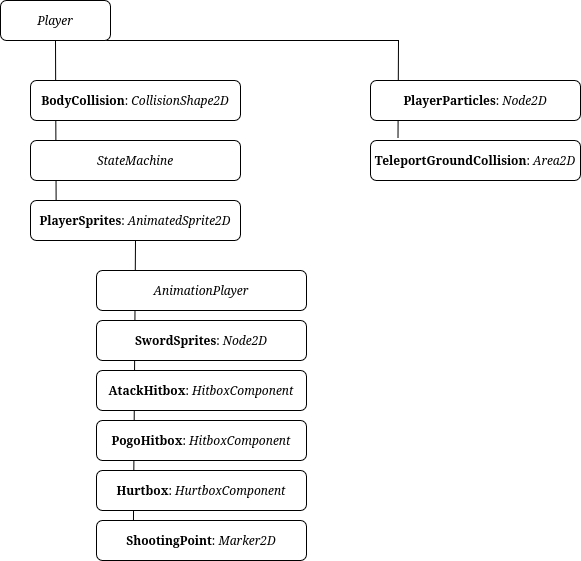
\includegraphics[scale=0.5]{img/player-architecture.drawio.png}
    \caption[Diagrama de la arquitectura del nodo Player]{Diagrama de la arquitectura del nodo Player. Se el tipo de nodo en cursiva y el nombre en negrita (si tuviera uno).}
    \label{fig:player-architecture-diagram}
\end{figure}

A continuación se repasarán los nodos principales de la figura \ref{fig:player-architecture-diagram}:
\begin{itemize}
    \item \textbf{BodyCollision}: Forma de colisión que usa \textit{CharacterBody2D} para detectar objetos sólidos del mundo.
    \item \textbf{StateMachine}: Nodo que gestiona la máquina de estados. Tiene como hijos un nodos tipo \textit{PlayerState} por cada estado.
    \item \textbf{PlayerSprites}: Aquí se crean y reproducen todas las animaciones de sprites del personaje. Como hijos figuran todos los nodos que deben ser sensibles a sus transformaciones de escala, como los detectores de colisiones (AtackHitbox, Hurtbox, etc.).
    \item \textbf{AnimationPlayer}: Si PlayerSprites reproduce visualmente la mayoría de animaciones, este nodo gestiona algunas más complejas, como la de ataque.
    \item \textbf{PlayerParticles}: Gestiona los sistemas de partículas del jugador.
    \item \textbf{TeleportGroundCollision}: Detector de colisiones auxiliar para la función de teletransporte.
\end{itemize}

\subsection{Máquina de estados}

Se usó la implementación de máquina de estados que se desarrollará en el apartado \ref{sec:state-machine}. El nodo \textit{StateMachine} contiene un nodo hijo por cada estado de Player. Estos nodos son del tipo \textit{PlayerState}. Cada nodo encapsula toda la lógica asociada a su estado. 

Por ejemplo se tiene el estado \textit{Move}, que gestiona el movimiento del jugador en el suelo. Sus responsabilidades serán, entre otras, inicializar la animación de caminar, recoger la entrada del mando para obtener la dirección de movimiento, y actualizar la posición del jugador.

A continuación se describen todos los estados:
\begin{itemize}
    \item \textbf{IDLE}: El jugador se encuentra en el suelo sin realizar ninguna acción.
    \item \textbf{MOVE}: El jugador se mueve en el suelo hacia izquierda o derecha.
    \item \textbf{JUMP}: El jugador salta y comienza a ganar altura.
    \item \textbf{FALL}: El jugador, suspendido en el aire, comienza a perder altura.
    \item \textbf{SUPER\_FALL}: El jugador lleva en caida libre durante un tiempo prolongado.
    \item \textbf{STOMP}: El jugador cae con fuerza al suelo después de caer durante un tiempo prolongado.
    \item \textbf{ATACK}: El jugador realiza un ataque con la espada.
    \item \textbf{PREPARE\_TELEPORT}: El jugador comienza a apuntar a algún lugar para teletransportarse.
    \item \textbf{RELEASE\_TELEPORT}: El jugador se teletransporta.
    \item \textbf{POGO}: El jugador coloca su espada bajo el personaje para rebotar en objetos.
    \item \textbf{HIT}: El jugador recibe un golpe.
    \item \textbf{DEAD}: El jugador no cuenta con más puntos de vida y es derrotado.
    \item \textbf{TALKING}: El jugador habla con un NPC.
\end{itemize}

Dado que la máquina de estados resultante es bastante compleja, representarla en un solo diagrama haría que fuese poco legible. En su lugar se representará por separado un diagrama para cada estado, en el que se indica a qué otros estados se puede transicionar partiendo desde ese y por qué motivo. Esto se puede consultar en las figuras \ref{fig:player-state-idle}, \ref{fig:player-state-jump}, \ref{fig:player-state-attack}, \ref{fig:player-state-pogo}, \ref{fig:player-state-move}, \ref{fig:player-state-fall}, \ref{fig:player-state-teleport} y \ref{fig:player-state-hit}.

\begin{figure}[h]
    \centering
    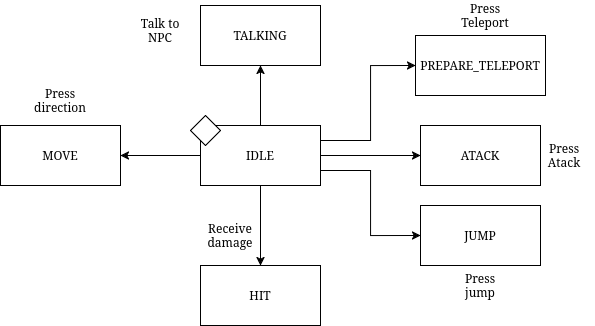
\includegraphics[scale=0.5]{img/player-sm-idle.drawio.png}
    \caption[Flujo de estados de IDLE, Player]{Diagrama de flujo de estados para el estado IDLE de Player.}
    \label{fig:player-state-idle}
\end{figure}

\begin{figure}[h]
    \centering
    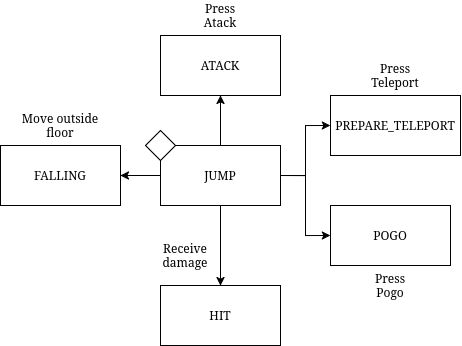
\includegraphics[scale=0.5]{img/player-sm-jump.drawio.png}
    \caption[Flujo de estados de JUMP, Player]{Diagrama de flujo de estados para el estado JUMP de Player.}
    \label{fig:player-state-jump}
\end{figure}

\begin{figure}[h]
    \centering
    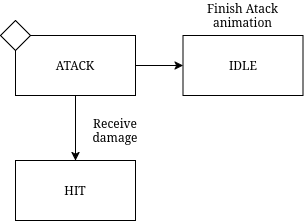
\includegraphics[scale=0.5]{img/player-sm-atack.drawio.png}
    \caption[Flujo de estados de ATTACK, Player]{Diagrama de flujo de estados para el estado ATTACK de Player.}
    \label{fig:player-state-attack}
\end{figure}

\begin{figure}[h]
    \centering
    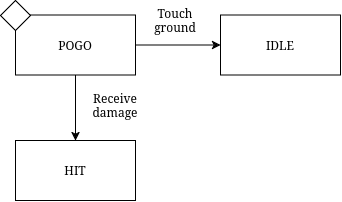
\includegraphics[scale=0.5]{img/player-sm-pogo.drawio.png}
    \caption[Flujo de estados de POGO, Player]{Diagrama de flujo de estados para el estado POGO de Player.}
    \label{fig:player-state-pogo}
\end{figure}

\begin{figure}[h]
    \centering
    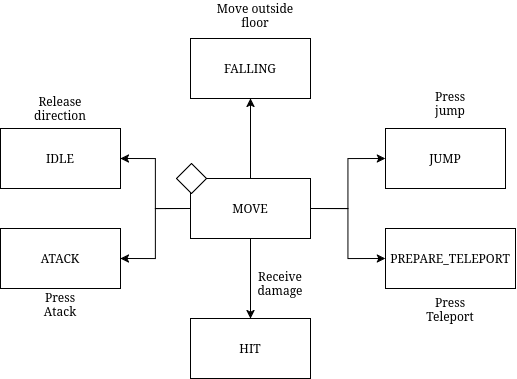
\includegraphics[scale=0.5]{img/player-sm-move.drawio.png}
    \caption[Flujo de estados de MOVE, Player]{Diagrama de flujo de estados para el estado MOVE de Player.}
    \label{fig:player-state-move}
\end{figure}

\begin{figure}[h]
    \centering
    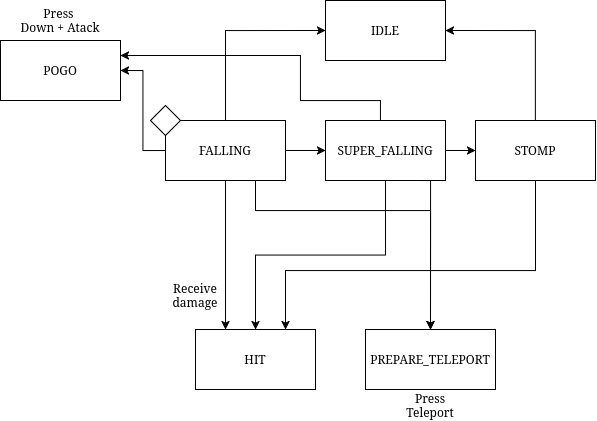
\includegraphics[scale=0.5]{img/player-sm-fall.drawio.png}
    \caption[Flujo de estados de FALL, Player]{Diagrama de flujo de estados para el estado FALL de Player.}
    \label{fig:player-state-fall}
\end{figure}

\begin{figure}[h]
    \centering
    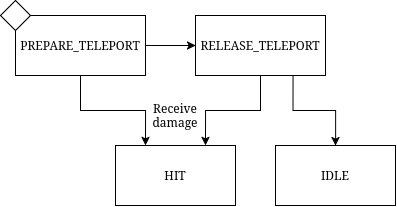
\includegraphics[scale=0.5]{img/player-sm-teleport.drawio.png}
    \caption[Flujo de estados de TELEPORT, Player]{Diagrama de flujo de estados para el estado TELEPORT de Player.}
    \label{fig:player-state-teleport}
\end{figure}

\begin{figure}[h]
    \centering
    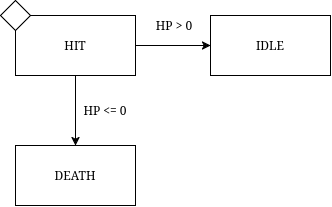
\includegraphics[scale=0.5]{img/player-sm-hit.drawio.png}
    \caption[Flujo de estados de HIT, Player]{Diagrama de flujo de estados para el estado HIT de Player.}
    \label{fig:player-state-hit}
\end{figure}


\subsection{Gestión de colisiones y físicas}

Podemos diferenciar dos tipos de colisiones que se necesitan gestionar: las que están relacionadas con la simulación de \textbf{físicas} (velocidad de movimiento y colisión con objetos sólidos) y las relacionadas con \textbf{interacciones} (cuando el jugador toca un enemigo debería recibir daño, cuando entra en contacto con un item debería recogerlo, etc).

Para las \textbf{físicas} se hace uso del motor por defecto de Godot. La gestión colisiones viene dada por el tipo \textit{CharacterBody2D}, del que hereda la escena Player. Este cuenta con una variable \textit{velocity}, un vector 2D que representa hacia dónde se mueve la escena y cómo de rápido. Al ejecut la función \textit{move\_and\_slide}, el jugador es desplazado, por lo que desde el script solo es necesario definir la dirección y magnitud deseado para el vector de velocidad. Si el nodo \textbf{BodyCollision} colisiona con un objeto sólido al desplazarse, se detiene en seco, y si lo hace con una pendiente, se desliza sobre ella.

Para las \textbf{interacciones} se hace uso del nodo \textit{Area2D}. Este permite definir un area de colisión y disparar una señal cada vez que un cuerpo u otro area entre dentro de esta (es decir, colisionen). La señal puede ser conectada a otros nodos para gestionar la interacción.

Es necesario poder discernir qué objeto es el que provoca la colisión. Por ejemplo, el área \textit{Hurtbox} dispara una señal cuando el jugador choca con un enemigo para restarle salud. Eso es algo que solo debe ocurrir si la colisión ha ocurrido con un enemigo, y no otro objeto. Para eso se hace uso de la propiedad de \textbf{capas y máscaras}. Todas las áreas y cuerpos en Godot deben declarar en qué cápa de las físicas se encuentran, y con qué otras capas puede interactuar (es decir, su \textit{máscara}). Para el caso de \textit{Hurtbox}, esta no necesitaría definir ninguna capa (ningún objeto necesita interactuar con esta) y en su máscara se define que interactuará con la capa \textit{EnemyAtack}, para poder detectarlos.

En el proyecto se definieron las siguientes capas:

\begin{itemize}
    \item \textbf{Player}: Capa dedicada al jugador.
    \item \textbf{Ground}: Contiene a todas las paredes, suelos y otros objetos sólidos.
    \item \textbf{PlayerAtack}: Ataques que emite el jugador.
    \item \textbf{Enemy}: Personajes enemigos.
    \item \textbf{EnemyAtack}: Cualquier objeto que pueda causar daño al jugador.
    \item \textbf{Breakable}: Objetos destruibles por el jugador.
    \item \textbf{Key}: Llaves que el jugador puede recoger.
\end{itemize}

Algunas de las interacciones que se definen en distintas escenas del proyecto son recurrentes: las áreas que reciben daño y las que producen daño. El jugador, los enemigos y algunos objetos destruibles o dañinos necesitan implementarlas. Por tanto es deseable encontrar una abstracción que evite el tener que codificarlas de forma redundante en cada una de esas escenas.

Cuando varias entidades necesitan implementar cierto comportamiento en el paradigma de la programación orientada a objetos, se resuelve por herencia. Se crea un super tipo con la funcionalidad del que heredarían los objetos pertinentes. Sin embargo, por la estructura en nodos de Godot y la necesidad particular de cada escena de heredar de según qué tipos, esta aproximación complicaría mucho el código del proyecto. En su lugar, se introduce el concepto de \textbf{componente}. Se entiende por componente una encapsulación de funcionalidad que puede ser inyectada en cualquier ente del proyecto. En Godot, esto se traduce en un nodo que se añade como hijo a cualquier escena que necesite implementar dicha funcionalidad.

Ante esta necesidad se implementaron los componentes \textbf{HitboxComponent} y \textbf{HurtboxComponent}. En desarrollo de videojuegos se denomina \textit{hitbox} al área de colisión que abarca el ataque de una actor. Por otro lado, \textit{hurtbox} es el área de colisión que define las zonas impactables de este, las que pueden recibir daño. En esencia, la hitbox de un ataque debe colisionar con una hurtbox de otro personaje para impactarle.

\textbf{HitboxComponent} hereda de Area2D. Define la función \textit{on\_atack\_detected}, que recibe como parámetro una \textit{HurtboxComponent}, y es conectada durante la instanciación del objeto a la señal \textit{\_on\_area\_entered}. Esta función recoge la dirección desde la que se recibió el golpe y llama a la función \textit{take\_damage} de su nodo padre.

La implementación de \textbf{HurtboxComponent} es vacía, dado que este objeto existe solo para tipar esta clase de área, y que las hitbox detecten únicamente a estas y no otra Area2D.

Por tanto, para implementar estos componentes en cualquier escena (por ejemplo, la de Player) se instancian los respectivos componentes, se añade como hijo una forma de colisión (requerida por el Area2D de la que se hereda) y el nodo padre deberá implementar la función \textit{take\_damage} para gestionar cómo se procesa el impacto. Por último, se indica una máscara para la hitbox (en este caso, Enemy) y una capa para la hurbox (Player).

En la figura \ref{fig:hit-components} se tiene una representación de este esquema para la escena Player. En otras escenas se realizaría de forma similar.

%TODO: Añadir diagrama para hitbox y hurtbox?

\begin{figure}[h]
    \centering
    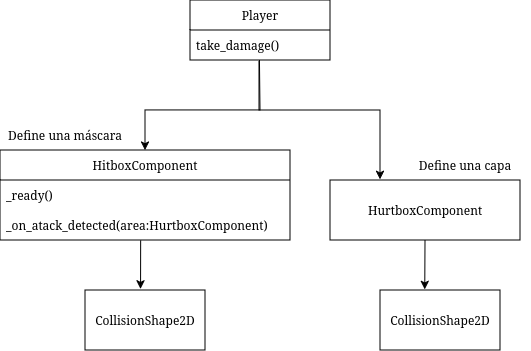
\includegraphics[scale=0.65]{img/hitbox-component-diagram.drawio.png}
    \caption[HitboxComponent y HurtboxComponent]{Diagrama de componentes HitboxComponent y HurtboxComponent para el nodo Player}
    \label{fig:hit-components}
\end{figure}


\subsection{Gestión de animaciones}

Las animaciones son gestionadas principalmente por el nodo \textit{AnimatedSprite2D}. Este permite definir una lista de animaciones que luego pueden ser llamadas desde el código. Una animación se define con un nombre y una colección de fotogramas. Es posible configurar la duración de cada uno de los fotogramas que la componen. Para crear los fotogramas, se hacen uso de \textit{spritesheets}.

Una \textbf{spritesheet} es una imagen dividida en cuadrículas que recoge una serie de fotogramas tematizados. Puede ser una paleta de bloques que se usan para dibujar el escenario, o en este caso, una colección de fotogramas de las animaciones de un personaje. En la figura \ref{fig:player-spritesheet} se muestra la correspondiente a Player.

\begin{figure}[h]
    \centering
    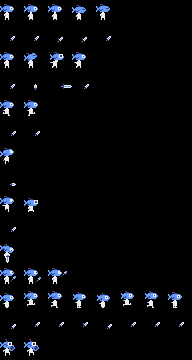
\includegraphics[scale=0.75]{img/player_spritesheet.png}
    \caption[Spritesheet de animaciones de Player]{Spritesheet de animaciones de Player}
    \label{fig:player-spritesheet}
\end{figure}

Como el jugador comienza el juego sin una espada y la obtiene más adelante, se han separado las animaciones del jugador en 2 nodos: \textit{PlayerSprites} y \textit{SwordSprites}. Esto se hace para evitar el duplicar todas las acciones del personaje, haciendo versiones con y sin espada. En la figura \ref{fig:player-spritesheet} se aprecia esta separación. Mientras no se consiga la espada, \textit{SwordSprites} se mantiene invisible.

Usando \textit{AnimatedSprite2D} se cubren la mayoría de animaciones, pero otras más complejas necesitan coordinar los fotogramas con la modificación de parámetros de la escena. Para esos casos se emplea \textit{AnimationPlayer}, un nodo más completo que permite crear animaciones en una timeline en la que se pueden ordenar e interpolar fotogramas, valores de parámetros y llamadas a funciones. Esto es necesario para, por ejemplo, modificar la trasparencia del sprite o activar y desactivar las áreas de colisión de la animación de ataque.

\subsection{Gestión de datos y parametrización}

En el script de Player se declaran una serie de variables con la etiqueta de Godot \textbf{@export}. Esta etiqueta hace que el valor de estas variables se pueda modificar desde la interfaz del motor y en tiempo de ejecución. Esto resulta muy práctico para realizar \textit{fine-tuning}, facilitando el ajuste de parámetros que afectan enormemente a la experiencia de juego como la velocidad de movimiento o altura del salto. La lista de parámetros es la siguiente:

\begin{itemize}
    \item \textbf{walking\_speed} (Float): Velocidad máxima al caminar.
    \item \textbf{walking\_acceleration} (Float): Aceleración al caminar.
    \item \textbf{walking\_deceleration} (Float): Deceleración al dejar de caminar.
    \item \textbf{air\_acceleration} (Float): Acelerazión horizontal en el aire.
    \item \textbf{pogo\_acceleration} (Float): Aceleración horizontal en el aire al realizar el pogo.
    \item \textbf{jump\_force} (Float): Fuerza de salto.
    \item \textbf{bounce\_force} (Float): Fuerza al rebotar con el pogo.
    \item \textbf{gravity\_jumping} (Float): Fuerza gravitatoria al ascender.
    \item \textbf{gravity\_falling} (Float): Fuerza gravitatoria al descender.
    \item \textbf{max\_fall\_speed} (Float): Velocidad máxima de caída.
\end{itemize}

Para gestionar las variables persistentes del jugador entre partidas se creó la estructura de datos \textbf{PlayerData}. Este es un recurso customizado de Godot y contiene información sobre las mejoras desbloqueadas y los puntos de salud máximos. Sus parámetros son:
%TODO: METER REFERENCIA A DONDE SE EXPLIQUEN LOS RECURSOS

\begin{itemize}
    \item \textbf{has\_sword\_update} (Boolean): Espada desboqueada.
    \item \textbf{has\_break\_update} (Boolean): Rompe-paredes desbloqueado.
    \item \textbf{has\_beam\_update} (Boolean): Disparo desbloqueado.
    \item \textbf{has\_pogo\_update} (Boolean): Pogo desbloqueado.
    \item \textbf{has\_teleport\_update} (Boolean): Teletransporte desbloqueado.
    \item \textbf{has\_key} (Boolean): Llave en posesión.
    \item \textbf{max\_health} (Int): Puntos máximos de salud.
\end{itemize}

Se añadió además una variable \textit{@export} tipo PlayerData. Al inicializar Player, si esta variable no es nula, en lugar de cargar los datos de guardado pertinentes, se cargan esos. Esta utilidad permite realizar una depuración y testeo del juego mucho más fácil.

\subsection{Mejora BEAM}

Esta mejora permite al jugador disparar un rayo desde su espada al atacar. El rayo avanza en línea recta y desaparece al transcurrir un tiempo o colisionar con un enemigo. Se creó la escena \textit{Beam} para gestionar este disparo. La arquitectura se puede observar en la figura \ref{fig:beam-architecture}. La escena hace uso de un nodo \textit{Line2D} para el efecto de estela.

\begin{figure}[h]
    \centering
    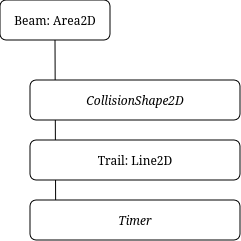
\includegraphics[scale=0.75]{img/beam-architecture.drawio.png}
    \caption[Arquitectura de escena Beam]{Arquitectura de escena Beam}
    \label{fig:beam-architecture}
\end{figure}

El ciclo de vida de los disparos es el siguiente:

\begin{enumerate}
    \item Player crea una instancia de Beam. Indica la dirección del disparo en función de su orientación y lo posiciona en el mismo punto que \textit{ShootingPoint}, nodo alineado con la espada para hacer ver que el disparo aparece en esta.
    \item Player añade este nodo como hijo de su padre (el nodo \textit{GameWorld}, consultar figura \ref{fig:proyect-architecture}).
    \item La escena Beam actualiza su posición en cada fotograma. Cuando colisiona con una pared o un enemigo, se destruye a si misma.
\end{enumerate}

\subsection{Mejora TELEPORT}

Para la mejora del teleport se creó la escena \textit{TeleportCrosshair}. Esta es responsable únicamente de avanzar en linea recta y reproducir una animación.

La escena hace uso de una \textit{Curve}, que se puede observar en la figura \ref{fig:teleport-curve}. Este recurso de Godot permite definir gráficamente una curva dentro de un dominio. En este caso se usa la curva para determinar la posición del \textit{crosshair} en función del tiempo transcurrido. Al tener una curva \textit{ease-out}, la escena iniciará con velocidad máxima y según avance irá frenando hasta detenerse. De esta forma se consigue un efecto más vistoso y satisfactorio.

\begin{figure}[h]
    \centering
    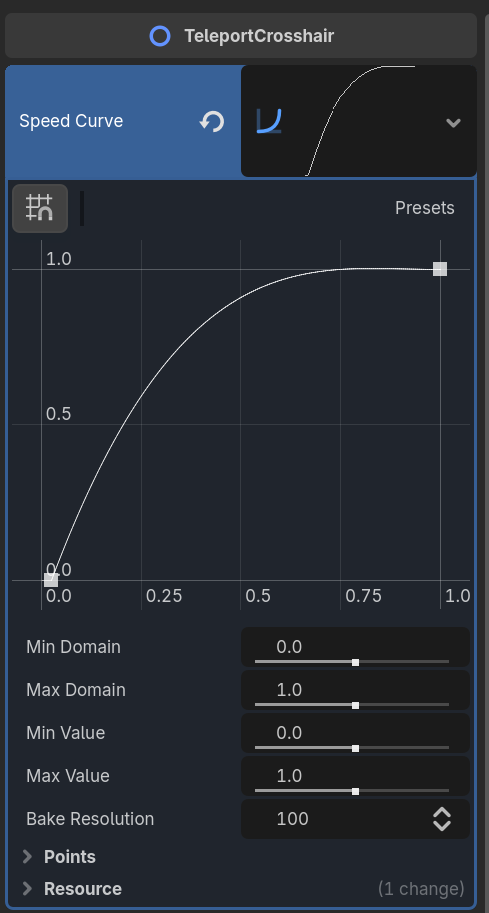
\includegraphics[scale=0.55]{img/teleport-curve.png}
    \caption[Recurso tipo Curve en Godot]{Recurso tipo Curve en Godot}
    \label{fig:teleport-curve}
\end{figure}

El esquema de funcionamiento es el siguiente:
\begin{enumerate}
    \item El jugador mantiene pulsado el botón de teletransporte, esto hace que se transicione al estado PREPARE\_TELEPORT.
    \item El estado PREPARE\_TELEPORT instancia una escena TeleportCrosshair. Indica la dirección apropiada en función de la orientación del jugador, y la añade como hijo de Player.
    \item Cuando el jugador suelta el botón de teletransporte, se transiciona al estado RELEASE\_TELEPORT.
    \item El estado RELEASE\_TELEPORT aplica una transformación a jugador para llevarlo al punto donde se encuentra el TeleportCrosshair y lo destruye.
    \item Si en el punto de teletransporte se detecta alguna colisión con el suelo, significa que ese punto no está libre, revierte la transformación. En caso contrario, el jugador se teletransporta con éxito.
\end{enumerate}

\subsection{Sistemas de partículas}

Los sistemas de partículas son una técnica empleada para recrear efectos visuales complejos como humo, fuego, explosiones o lluvia entre otros. Hacen uso de partículas, elementos cuyo aspecto y comportamiento se programa para lograr los efectos deseados. Es indispensable que el coste computacional de crear y destruir partículas sea muy liviano, ya que se necesita hacer uso de grandes conjuntos para lograr los efectos deseados.

Godot cuenta con los nodos CPUParticle2D y GPUParticle2D, para la creación de sistemas de partículas con la CPU y GPU respectivamente. El primero es menos eficiente y ofrece menos posibilidades que el segundo, pero a cambio ofrece una mejor compatibilidad a la hora de exportar a plataformas como navegador web. Se decidió usar CPUParticle2D ya que los sistemas que se necesitaban implementar en el proyecto no tenían un coste computacional elevado. Así se asegura una mejor compatibilidad.

Al configurar cada sistema de partículas se pueden establecer parámetros como la textura, la gravedad, la velocidad inicial, variación en color, variación en tamaño, rotación, etc. Se desarrollaron partículas para cuando el jugador es golpeado, para cuando cae desde muy alto y para cuando muere. Todos los sistemas de partículas se agruparon bajo el nodo \textit{PlayerParticles} y se añadió un script a este para gestionar su instanciación.

%\subsection{Técnicas avanzadas} %coyote time, salto

\section{Gestión de niveles y mapeado}

Como se mencionó en apartados anteriores, la escena \textit{GameWorld} es la responsable de gestionar los espacios virtuales que componen el juego (es decir, los niveles). Esta escena se integró con la funcionalidad de \textbf{Metroidvania System}\cite{metsys} (abreviado como \textit{MetSys}), un plugin de Godot. MetSys contiene una colección de herramientas recurrentes en el desarrollo de juegos metroidvania. Facilita el proceso de diseño de mapa, procesa la navegación entre instancias del juego, gestiona las interfaces de usuario relacionadas con el mapa y se ocupa de parte de los datos de guardado.

%Menú de diseño de mapas

MetSys añade un editor de mapa integrado en Godot, se puede ver en la figura \ref{fig:metsys-map-editor}. Desde esta interfaz se puede diseñar visualmente todo el mapeado del juego. El mapa está compuesto de \textbf{salas}, que se crean y se disponen dibujando sobre el editor.

\begin{figure}[h]
    \centering
    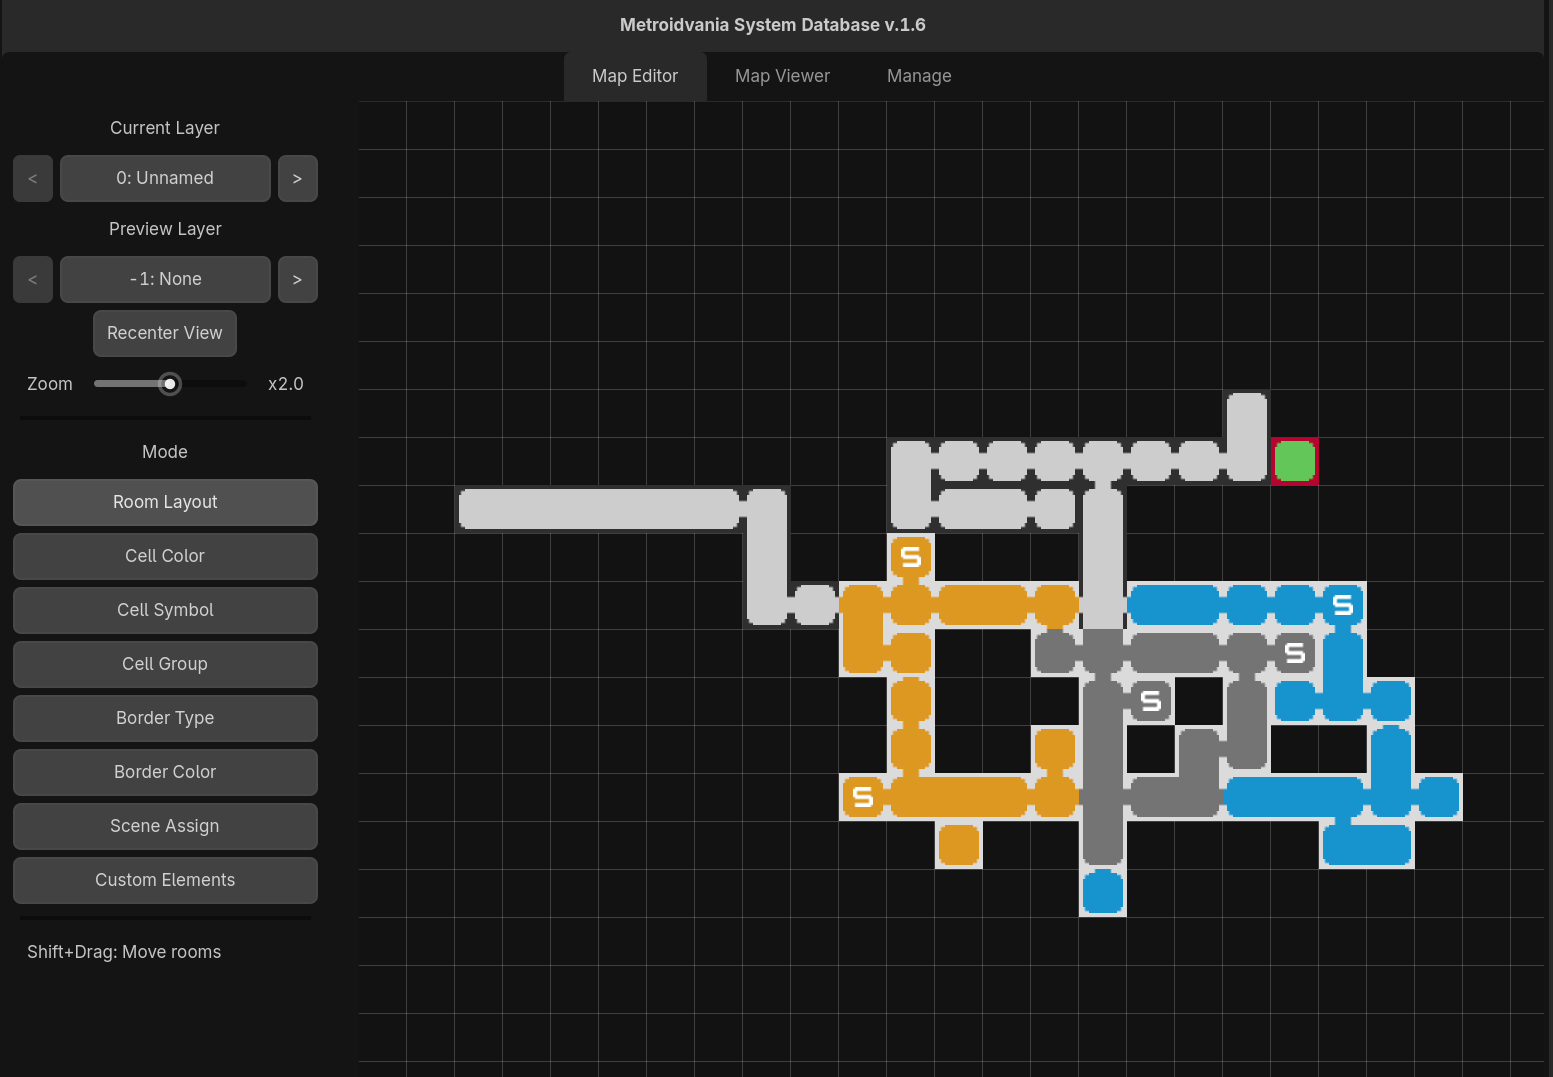
\includegraphics[scale=0.30]{img/metsys-map-menu.png}
    \caption[Editor de mapas de MetSys]{Editor de mapas de MetSys.}
    \label{fig:metsys-map-editor}
\end{figure}

\subsection{Salas y células}

Una \textbf{sala} en MetSys es un espacio virtual que puede ser recorrido por el jugador. Este se asigna a una escena de Godot, la cual describe su contenido. Las salas están colocadas en unas coordenadas del mapa y tienen otras salas adyacentes. Desde el editor se puede definir el color con el que se representará y su tipo de borde (abierto o cerrado) para con cada una de sus salas adyacentes.

Una sala está dividida en \textbf{células}. Cada célula es un cuadrante en las coordenadas del mapa y tienen una resolución fija. Es posible tener una sala de una sola célula. Se decidió que para este proyecto la resolución de una célula fuera de \textit{256x224} píxeles, la misma que la ventana del ejecutable. Esto se debe a que en el diseño de niveles se contemplaban principalmente salas de una sola pantalla (sin desplazamiento), y pocas pantallas con desplazamiento, por lo que no era necesario desgranar las salas en secciones menores y así se facilita la iteración sobre el diseño del mapa.

%Explicar el elemento de room, qué compone RoomTemplate.tscn, cómo se crea una sala

Al definir en el editor una sala, se le asigna una escena. Se configuró el plugin para asignar por defecto \textit{RoomTemplate}, una escena de tipo Nodo2D que contiene los elementos mínimos necesarios para construir salas en este proyecto. Esta se compone de los siguientes nodos:

\begin{itemize}
    \item \textbf{RoomInstance}: Nodo de MetSys que permite la integración de la escena con la base de datos del mapa. Permite previsualizar escenas adyacentes desde el editor, y ofrece utilidades para interactuar con el mapa en tiempo de ejecución.
    \item \textbf{TileMapLayer}: Nodo de Godot que permite la creación de mapas 2D basados en cuadrículas a través de un \textit{TileSet}, una librería de \textit{tiles}. Los tiles son la mínima unidad de bloque en forma de imagen con la que se construye el mapa.
    \item \textbf{RoomRespawn}: Nodo de tipo Marker2D. \textit{GameWorld} toma su posición dentro de la escena de referencia para saber dónde debería aparecer el jugador si carga la partida en una sala dada.
\end{itemize}

Al añadir una sala al mapa, se crea su escena tomando \textit{RoomTemplate} como base, se dibuja a mano su topografía en el TileMapLayer, y se añaden otros elementos que pudieran pertenecer a la escena como enemigos, objetos o NPCs. En la figura \ref{fig:completed-room} se tiene un ejemplo de una sala completa.

\begin{figure}[h]
    \centering
    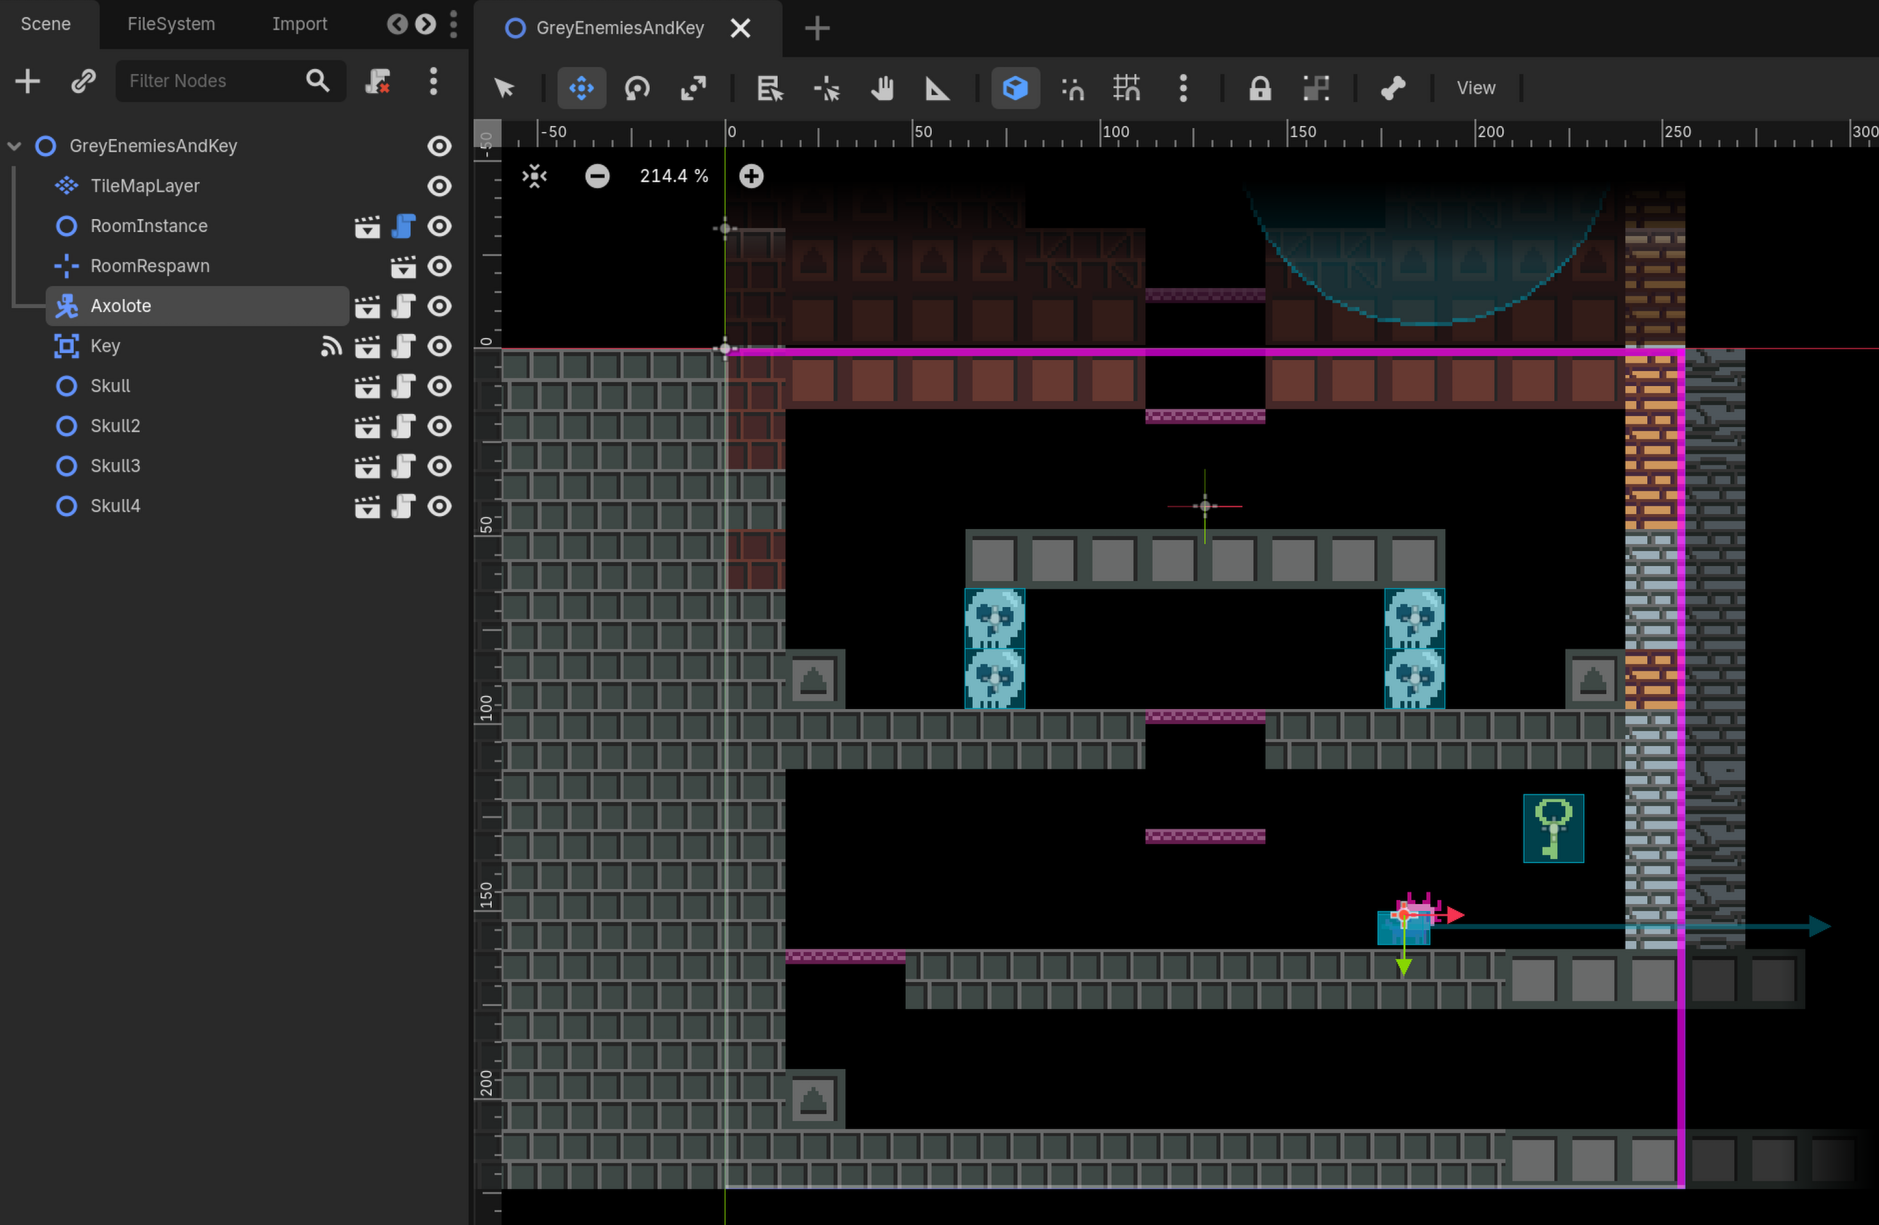
\includegraphics[scale=0.25]{img/complete-room.png}
    \caption[Sala completa en el editor de Godot.]{Sala completa en el editor de Godot. A la derecha se tienen todos los nodos que lo componen. Arriba y a la derecha se previsualizan las salas adyacentes.}
    \label{fig:completed-room}
\end{figure}

\subsection{Creación de TileSet}

Para configurar un TileSet es necesario disponer de un \textit{tile atlas}, una imagen que recoge todos los tiles que pertenecen a una zona del juego. Por ejemplo, se podría tener un \textit{tile atlas de los niveles del bosque}. Por el alcance de este proyecto, en un solo atlas se recogen todos los tiles del juego. Se puede observar en la figura \ref{fig:tile-atlas}. Para producirlo tanto este como el resto de recursos visuales del proyecto se empleó el editor de imágenes \textit{pixel art} Aseprite \cite{aseprite}.

\begin{figure}[h]
    \centering
    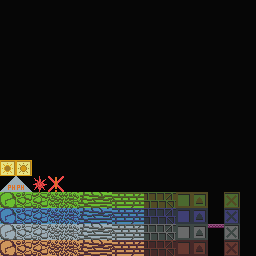
\includegraphics[scale=0.60]{img/tilemap.png}
    \caption[Tile atlas del proyecto.]{Tile atlas del proyecto.}
    \label{fig:tile-atlas}
\end{figure}

El atlas está dividido en regiones del mismo tamaño (los tiles). Es posible que un elemento del juego ocupe varios tiles si fuera muy grande. El TileSet de Godot se configura para reconocer estas regiones y poder asignarle propiedades de forma individual.

Una de las propiedades a configurar son las capas de física. Para cada tile se puede definir un área de colisión asignada a una capa de físicas del proyecto. Se le asignó la capa \textit{Ground} a los suelos y paredes para que colisionen con las físicas del jugador y los enemigos. Por otro lado se usó la capa \textit{EnemyAtack} en un tile para hacer que el jugador se dañe al tocarla.

También puede asignarse a cada tile una \textit{capa de navegación}. Estas capas se emplean para definir el áreas que pueden usarse para implementar técnicas de \textit{pathfinding}. Esto se empleó para desarrollar un enemigo que navega los niveles evitando chocar con paredes mientras persigue al jugador, como se explicará más adelante. Se creó una únca capa de navegación y se asignó a un tile vacío que se usará para definir las áreas por las que podrá navegar este enemigo.


\subsection{Escena GameWorld}

%GameWorld hereda de MetSysGame, arquitectura de la escena

La arquitectura de la escena GameWorld se puede ver en la figura \ref{fig:game-world-architecture}. Esta hereda de \textit{MetSysGame}, un script de MetSys responsable de la gestión del mapa y de localizar al jugador. La función que desempeñan el resto de nodos que la componen son las siguientes:

\begin{itemize}
    \item \textbf{Player}: Escena del jugador.
    \item \textbf{KeyManager}: Se encarga de gestionar la instanciación del objeto \textit{Key} al cambiar de sala.
    \item \textbf{PlayerUI}: Escena que muestra el marco del juego y la vida actual del jugador.
    \item \textbf{MapMenu}: Contiene el menú del mapa y el del mini-mapa.
\end{itemize}

\begin{figure}[h]
    \centering
    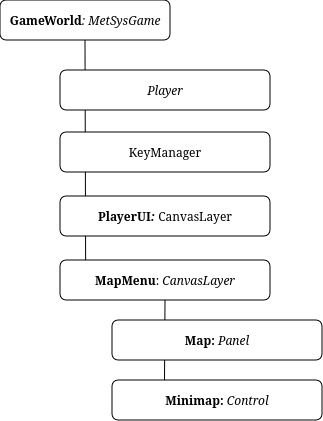
\includegraphics[scale=0.60]{img/gameworld-architecture.drawio.png}
    \caption[Arquitectura de escena de GameWorld.]{Arquitectura de escena de GameWorld.}
    \label{fig:game-world-architecture}
\end{figure}

%Explicar flujo de carga de GameWorld

A la hora de instanciar GameWorld, esta realiza los siguientes pasos:

\begin{enumerate}
    \item En caso de haber datos de guardado, carga en la base de datos de MetSys aquellos relacionados con la gestión del mapa: los objetos recogidos, las salas exploradas y los eventos registrados.
    \item Designa a la escena \textit{Player} como la escena del jugador de MetSys para que pueda rastrear su posición en las coordenadas globales del mapa.
    \item Delega en MetSys la carga de la habitación en la que comenzará el jugador obtenida del autoload \textit{DataManager}.
\end{enumerate}

De esta forma, MetSys tiene presente la posición del jugador dentro de una sala, y esa sala está posicionada en unas coordenadas del mapa. Al salirse el jugador de esas coordenadas, se dispara automáticamente la carga de la escena adyacente y la destrucción de la escena anterior. El resto de funcionalidades de MetSys ya pueden ser usadas y se integrarán con GameWorld sin necesitar de ninguna implementación extra.

Los nodos \textit{Map} y \textit{Minimap} están asignados a scripts de MetSys para renderizar el mapa creado previamente a través del editor gráfico. Estos centran su vista en las coordenadas del jugador automáticamente. Las salas que ya han sido visitadas son dibujadas en el mapa, mientras que el resto no aparecen. En la figura \ref{fig:map-menu} se puede ver el menú de visualización del mapa.

\begin{figure}[h]
    \centering
    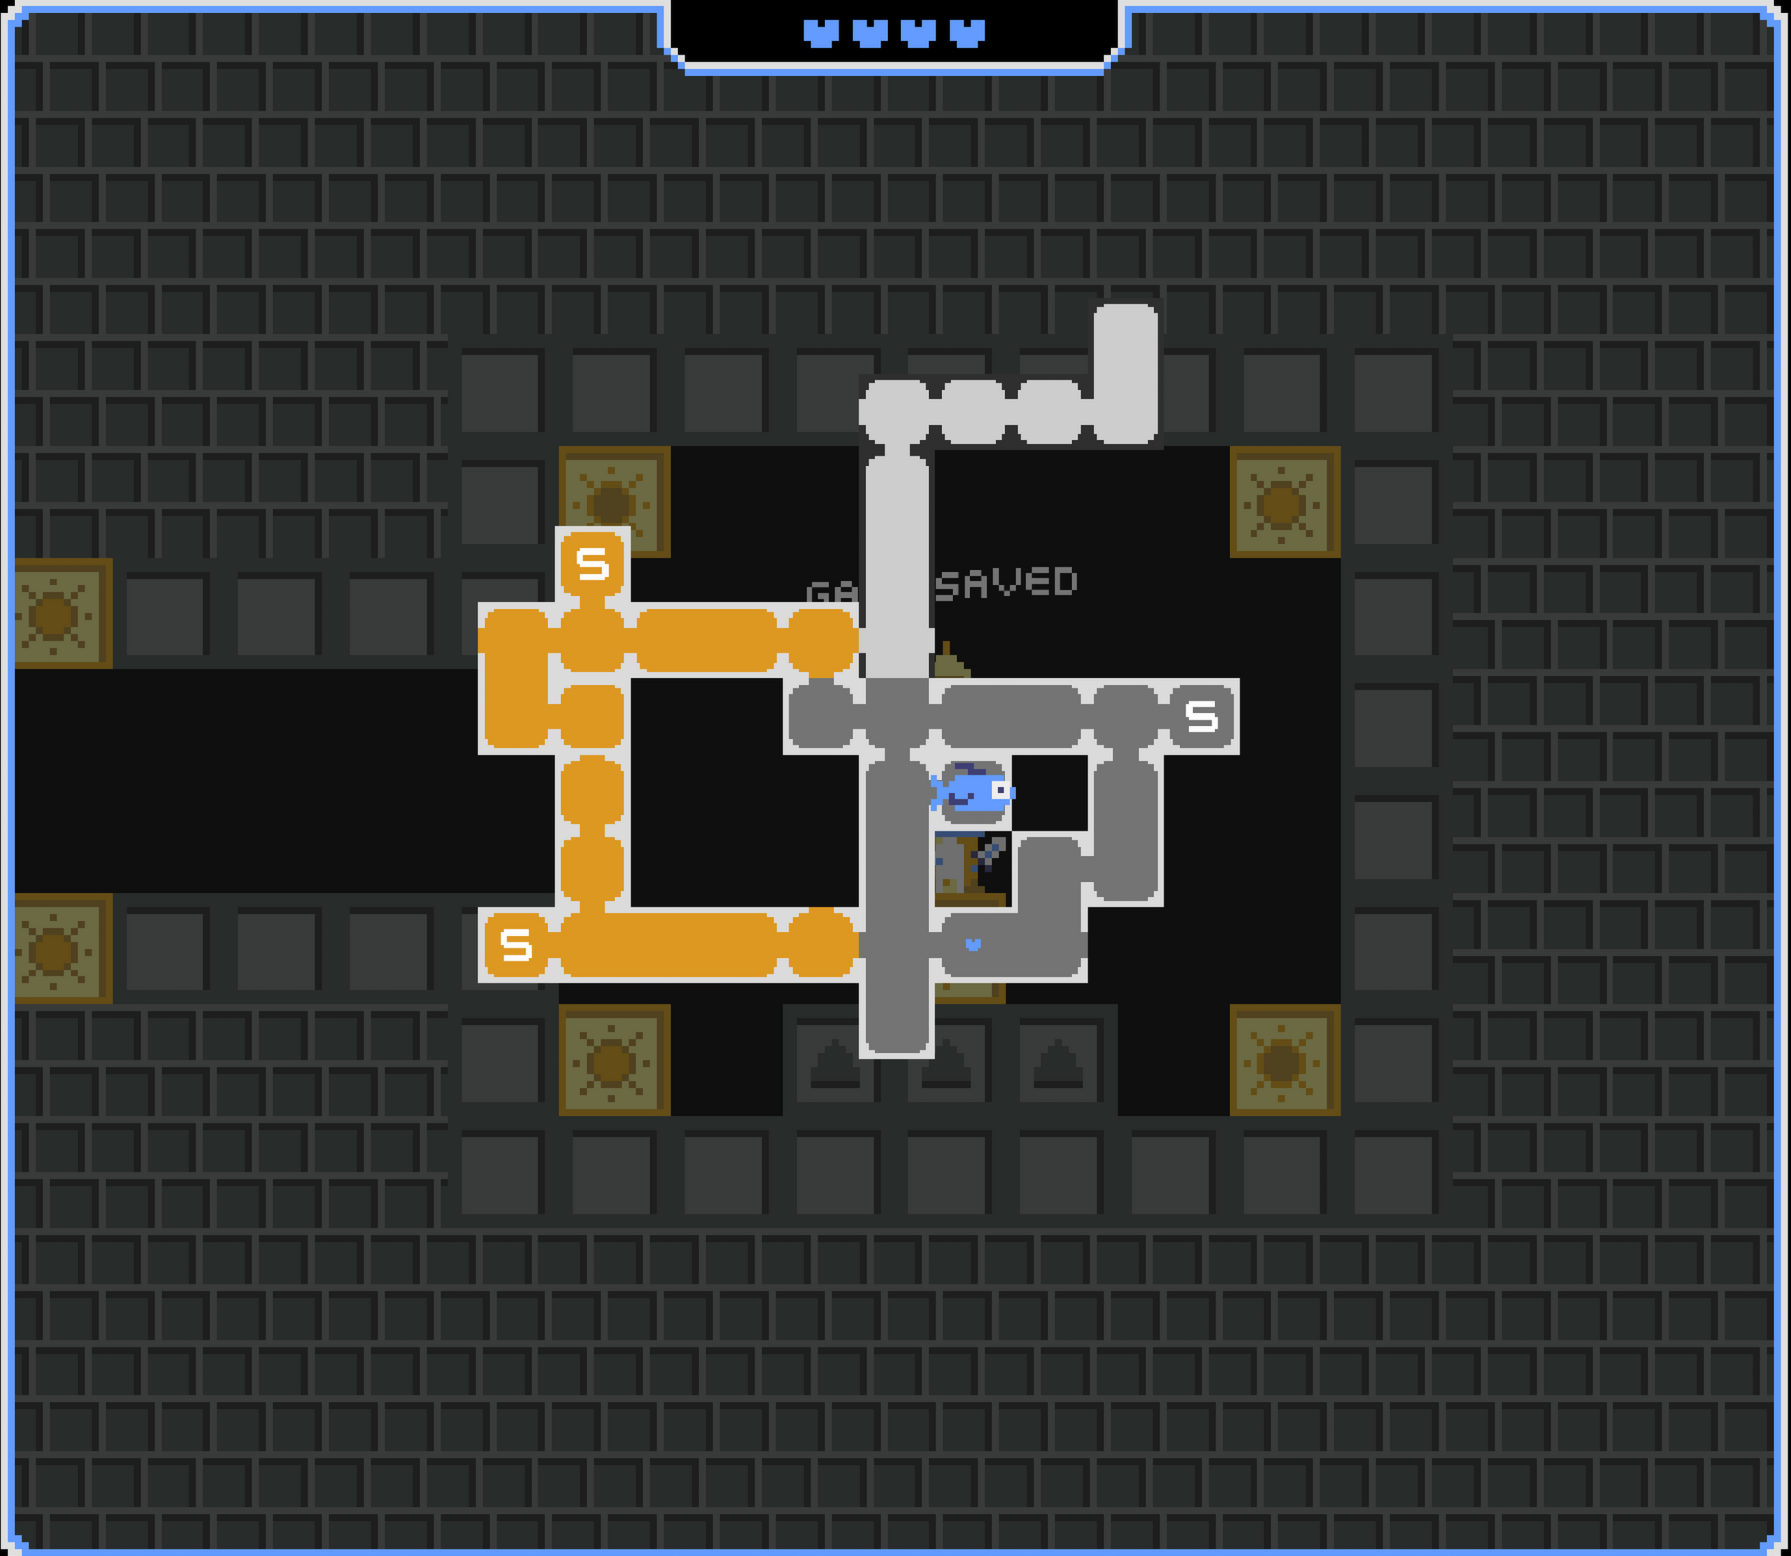
\includegraphics[scale=0.25]{img/map-menu.png}
    \caption[Interfaz de mapa del juego.]{Interfaz de mapa del juego. Se muestran las salas que el jugador ya ha visitado. Además, se marcan las salas con puntos de guardado y aquellas donde se ha conseguido algún objeto.}
    \label{fig:map-menu}
\end{figure}

\subsection{Gestión de items}

%Objetos pickable

En el juego hay objetos que el jugador puede recoger por el mapa como las mejoras que dotan al personaje de nuevas habilidades o corazones que aumentan su vida máxima. Una vez recogidos, estos no deben volver a ser instanciados en sus respectivas salas. Además, es de interés que se marquen con un icono las salas en las que se encuentran esos objetos para que el jugador interprete fácilmente el mapa.

MetSys cuenta con funciones para registrar nodos como \textit{storable object} (objeto que se puede recoger). De esta forma, los objetos recogibles se marcan a si mismos como tal durante su creación. Al entrar en contacto con el jugador, registran que ya han sido obtenidos. La próxima vez que se entre a la sala donde se encontraba, MetSys no lo instanciará.

Se crearon las clases \textbf{Collectible} y \textbf{CollectibleWithMarker} para gestionar esta interacción con MetSys. Los distintos objetos del juego heredan de uno de estos dos tipos en función de si se marcarán en el mapa o no. Estos se comunicarán con el autoload MetSys para incluirse en la base de datos del mapa. En la figura \ref{fig:collectible-diagram} se puede ver un esquema del funcionamiento.

\begin{figure}[h]
    \centering
    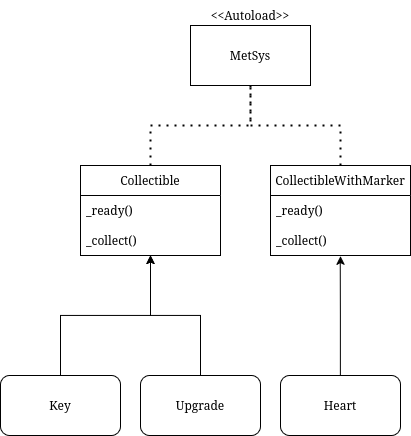
\includegraphics[scale=0.60]{img/collectible-diagram.drawio.png}
    \caption[Diagrama para las clases Collectible y CollectibleWithMarker]{Diagrama para las clases Collectible y CollectibleWithMarker}
    \label{fig:collectible-diagram}
\end{figure}

%Explicar problemática de llaves y KeyManager

Uno de los objetos que el jugador puede recojer son llaves (escena \textit{Key}). Cuando el jugador toca una llave, esta le sigue flotando por el mapa. Cuando está lo suficientemente cerca de una puerta cerrada, la abre y desaparece. Esto crea un problema con el funcionamiento de MetSys y las salas. El plugin solo permite transportar de una sala a otra al jugador. Al hacerlo, no es consistente con las coordenadas globales de Godot. Es decir, si el jugador está en el borde de la sala A (coordenadas (100,0)) y se mueve 10 píxeles a la derecha para pasar a la sala B, es posible que su posición no sea (110, 0) al completarse la transición.

Para el jugador esto no es ningún problema porque MetSys gestiona los límites de la cámara del jugador para que este cambio interno no sea perceptible al ojo humano. Pero si se quiere transportar una llave de una sala a otra haciendo parecer que sigue al jugador, esta tendrá un comportamiento errático.

Para solucionarlo se añádió a GameWorld la el nodo \textit{KeyManager} cuya implementación se detalla a continuación. En la figura \ref{fig:keymanager-flow} se tiene un esquema del siguiente flujo:

\begin{enumerate}
    \item El jugador obtiene una llave, haciéndola hija suya. Player emite un evento a través de GameEvent, el cual consume KeyManager. Así este obtiene una referencia a Player y a Key. La escena Key es responsable de perseguir la posición del jugador por la habitación actual.
    \item GameWorld emite una señal avisando que se ha comenzado una transición entre habitaciones. KeyManager guarda el vector de distancia entre Player y Key. A continuación, corta a Key de la escena Player para hacerla hija de KeyManager.
    \item La escena finaliza la transición. KeyManager devuelve a Player la llave y la coloca a la distancia a la que se encontraba respecto al jugador previa a la transición.
    \item Al abrir la llave una puerta, esta lo notifica a través de GameEvent. KeyManager consume esa señal y elimina la referencia a Key.
\end{enumerate}

\begin{figure}[h]
    \centering
    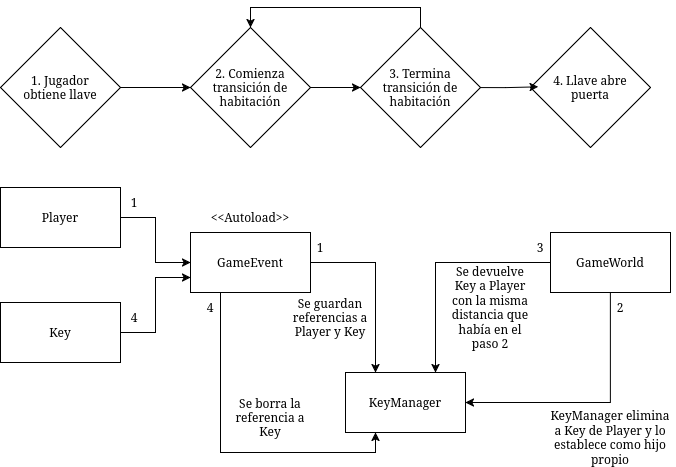
\includegraphics[scale=0.55]{img/key-manager-flow.drawio.png}
    \caption[Flujo del funcionamiento de KeyManager]{Flujo del funcionamiento de KeyManager.}
    \label{fig:keymanager-flow}
\end{figure}

\section{Enemigos}

% Enemy y EnemyCharacter
El juego cuenta con 5 tipos de enemigos distintos a los que tendrá que enfrentarse el jugador. Cada uno de ellos tiene un aspecto único y exhibe comportamientos distintos. Para implementarlos se crearon dos clases que actuan a modo de interfaz, \textit{Enemy} y \textit{EnemyCharacter}. En funcion de las necesidades de cada enemigo sus nodos raíz heredarán de un tipo u otro. En la figura \ref{fig:enemy-diagram} se muestra este esquema en un diagrama de clases:

\begin{itemize}
    \item \textbf{Enemy}: Hereda de Node2D. Se usa en enemigos con patrones de movimiento fijos y simples que no interactúan con las físicas del juego.
    \item \textbf{EnemyCharacter}: Se emplea en enemigos con comportamientos más complejos que requieren las funcionalidades de CharacterBody2D, del cual hereda la clase. Por ejemplo, modificar su trayectoria, velocidad o reaccionar a la gravedad.
\end{itemize}

\begin{figure}[h]
    \centering
    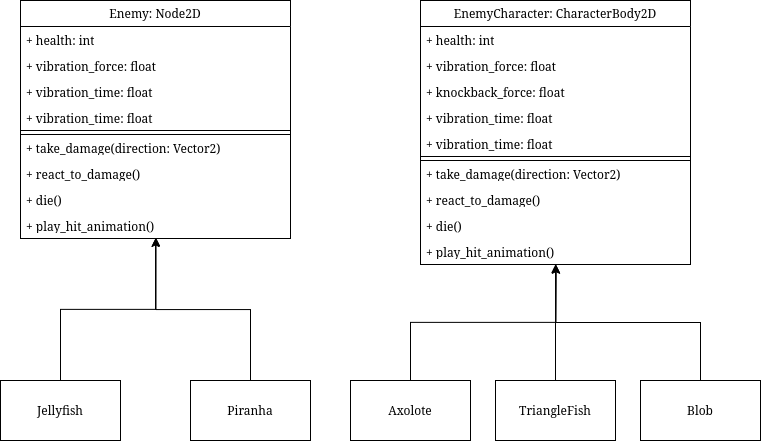
\includegraphics[scale=0.50]{img/enemy-diagram.drawio.png}
    \caption[Diagrama de clases de los enemigos del juego]{Diagrama de clases de los enemigos del juego.}
    \label{fig:enemy-diagram}
\end{figure}

Para implementar las \textit{hitbox} y \textit{hurtbox} de los enemigos se usa el componente \textit{HitboxComponent} y \textit{HurtboxComponent} que se explicó en la sección de Player de este capítulo. Este se añade en la escena de cada enemigo y se configura con sus capas y/o máscara correspondiente. Todos ellos cuentan además con un nodo AnimationPlayer para reproducir efectos visuales al ser golpeados y al morir. Estos efectos son comunes para todos los enemigos y comparten un \textit{recurso} de Godot, de forma que si en alguna escena se modifica, se actualiza en el resto.

A continuación se describirán las características de cada enemigo y los detalles concretos de su implementación.

    % Medusa

\subsection{Jellyfish}

Este enemigo es una medusa que oscila siguiendo una trayectoria circular alrededor de un punto. Hereda de la clase \textit{Enemy}. Su \textbf{radio} y \textbf{velocidad de rotación} están indicadas como variables \textit{@export}, por lo que se pueden ajustar desde la interfaz de Godot, agilizando el diseño de los niveles. Su arquitectura se muestra en la figura \ref{fig:jellyfish-architecture}.

Durante su instanciación, el nodo \textit{JellyPosition} se desplaza una longitud igual al radio en el eje y. En cada fotograma se aplica una rotación a \textit{RotationAxis}, consiguiendo que \textit{JellyPosition} describa una circunferencia. Por último, se coloca en la posición de este al nodo \textit{Character}.

\begin{figure}[h]
    \centering
    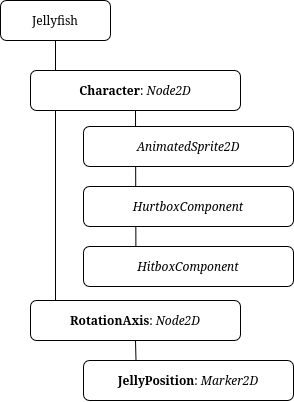
\includegraphics[scale=0.50]{img/jellyfish-architecture.drawio.png}
    \caption[Arquitectura de la escena Jellyfish]{Arquitectura de la escena Jellyfish.}
    \label{fig:jellyfish-architecture}
\end{figure}

    % Piraña

\subsection{Piranha}

Se trata de una piraña con una gran boca que recorre un camino lineal de ida y vuelta entre dos puntos. Hereda de la clase \textit{Enemy}. Se puede configurar su velocidad en cada instancia con una variable \textit{@export}. Se puede ver su arquitectura en la figura \ref{fig:piranha-architecture}.

Cada vez que se instancia esta escena en alguna sala, se deben posicionar los nodos \textit{StartPoint} y \textit{EndPoint}. La escena registra las coordenadas globales de estos puntos como inicio y destino, e interpola la posición del enemigo en función de la velocidad.


\begin{figure}[h]
    \centering
    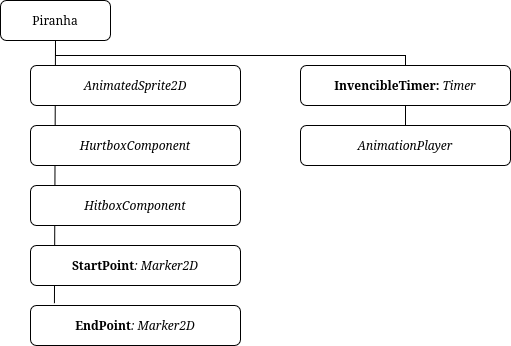
\includegraphics[scale=0.50]{img/piranha-architecture.drawio.png}
    \caption[Arquitectura de la escena Piranha]{Arquitectura de la escena Piranha.}
    \label{fig:piranha-architecture}
\end{figure}

    % Blob

\subsection{Blob}

Este ememigo es un pez abisal que se arrastra por el suelo. Hereda de \textit{EnemyCharacter}. Avanza en linea recta hasta toparse con un muro o hasta llegar al borde de una plataforma. Entonces, da media vuelta y avanza hacia al lado contrario. En la figura \ref{fig:blob-architecture} se muestra la arquitectura del nodo.

Debido a que su patrón de comportamiento es muy simple se decidió no implementar una máquina de estados. Se muestra un diagrama de su rutina en la figura \ref{fig:blob-flow}.

Los dos nodos \textit{Raycast2D} emplean una técnica de raycasting para detectar si el enemigo ha chocado contra una pared o está a punto de caer por un saliente. Esta técnica consiste en trazar desde un punto un rayo con cierta dirección y longitud. El rayo devuelve información sobre los objetos con los que ha colisionado. En este caso, se configuraron ambos raycast para colisionar con la capa \textit{Ground} (suelo, paredes, etc.). Si el primer rayo colisiona con algo, se infiere que está frente a una pared, por lo que deberá girar. De igual forma, si el segundo raycast, que apunta hacia abajo, no colisiona con nada, significa que hay un saliente y se volteará.

\begin{figure}[h]
    \centering
    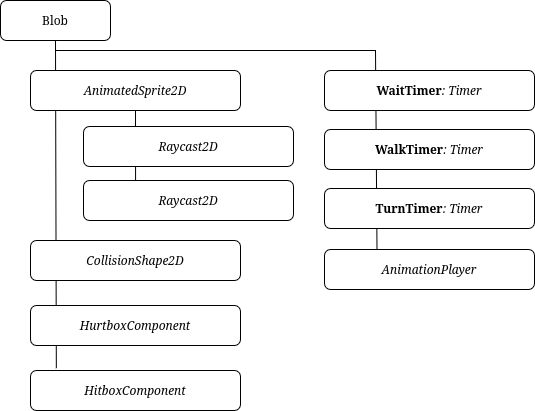
\includegraphics[scale=0.50]{img/blob-architecture.drawio.png}
    \caption[Arquitectura de la escena Blob]{Arquitectura de la escena Blob.}
    \label{fig:blob-architecture}
\end{figure}

\begin{figure}[h]
    \centering
    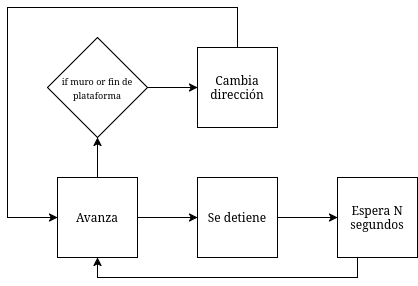
\includegraphics[scale=0.50]{img/blob-behaivour.drawio.png}
    \caption[Flujo de comportamiento de la escena Blob]{Flujo de comportamiento de la escena Blob.}
    \label{fig:blob-flow}
\end{figure}

    % Axolote

\subsection{Axolote}

Este enemigo es un ajolote mexicano. Camina por el suelo y se lanzará corriendo hacia el jugador a gran velocidad en caso de detectarle. Hereda de \textit{EnemyCharacter} e implementa una máquina de estados para codificar su comportamiento. Su arquitectura se muestra en la figura \ref{fig:axolote-architecture}. 

Para la máquina de estados se usó la misma implementación que la clase \textit{Player}. El diagrama de esta se muestra en la figura \ref{fig:axolote-state-machine}. Los estados son los siguientes:

\begin{itemize}
    \item \textbf{MOVE}: Estado inicial. El ajolote se mueve en una dirección hasta choca con una pared, momento en el que se da la vuelta.
    \item \textbf{SURPRISE}: Cuando tiene visión directa del jugador, se para en seco y se sorprende.
    \item \textbf{RUN}: Tras sorprenderse empieza a correr. Si choca contra un muro, se da la vuelta. Si al darse la vuelta no está viendo al jugador, vuelve a andar.
    \item \textbf{HIT}: Cuando recibe un golpe sale disparado algunos metros en el aire.
    \item \textbf{DEAD}: Cuando se queda sin puntos de vida (HP) reproduce su animación de muerte y se destruye la escena.
\end{itemize}

Este enemigo usa raycasting para saber cuando tiene delante un muro y debe girar. También lo usa para saber si el jugador está delante suya, creando el efecto de sorpresa al verlo.

\begin{figure}[h]
    \centering
    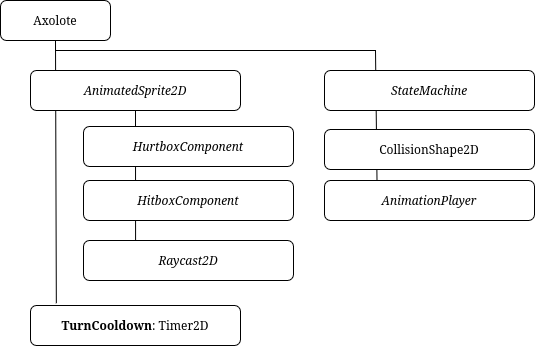
\includegraphics[scale=0.50]{img/axolote-architecture.drawio.png}
    \caption[Arquitectura de la escena Axolote]{Arquitectura de la escena Axolote.}
    \label{fig:axolote-architecture}
\end{figure}

\begin{figure}[h]
    \centering
    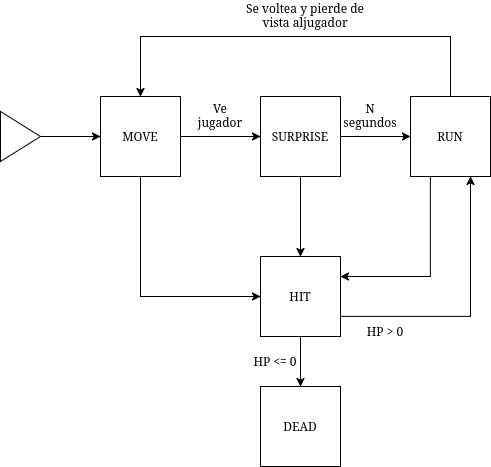
\includegraphics[scale=0.50]{img/axolote-state-machine.drawio.png}
    \caption[Máquina de estados para el enemigo Axolote]{Máquina de estados para el enemigo Axolote.}
    \label{fig:axolote-state-machine}
\end{figure}

    % Triangle

\subsection{Triangle Fish}

Este pez triangular se desplaza flotando por el aire. Aparece estando dormido. Si el jugador se acerca lo suficiente, se despertará. Tras eso, en el momento que vea al jugador, empezará a perseguirlo. Su arquitectura puede verse en la figura \ref{fig:triangle-architecture}. Esta clase hereda de \textit{EnemyCharacter} e implementa una máquina de estados que se ilustra en la figura \ref{fig:triangle-state-machine}. Los estados son los siguientes:

\begin{itemize}
    \item \textbf{SLEEP}: El enemigo comienza dormido. En este estado no se mueve. Si el jugador se mueve lo suficientemente cerca, se despertará.
    \item \textbf{WATCH}: El enemigo ha escuchado al jugador y ha despertado. Pero permanecerá inmóvil apuntando con un raycast en dirección al jugador hasta que tena una visión directa de este.
    \item \textbf{CHASE}: Comienza a perseguir al jugador aplicando una algoritmo de pathfinding para navegar el mapa.
    \item \textbf{HIT}: Se ha recibido un golpe. Retrocede durante unos instantes.
    \item \textbf{DEAD}: Cuando se queda sin puntos de vida (HP) reproduce su animación de muerte y se destruye la escena.
\end{itemize}

\begin{figure}[h]
    \centering
    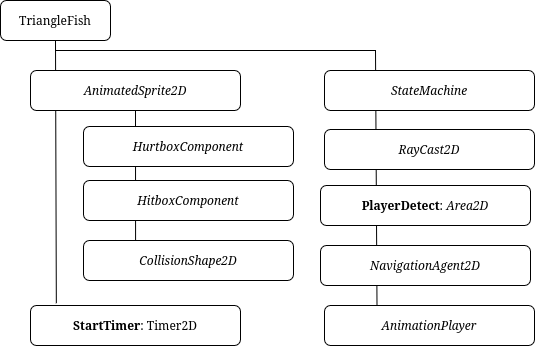
\includegraphics[scale=0.50]{img/trianglefish-architecture.drawio.png}
    \caption[Arquitectura de la escena TriangleFish]{Arquitectura de la escena TriangleFish.}
    \label{fig:triangle-architecture}
\end{figure}

\begin{figure}[h]
    \centering
    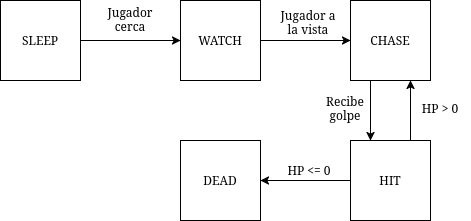
\includegraphics[scale=0.50]{img/triangle-state-machine.drawio.png}
    \caption[Máquina de estados para el enemigo Triangle Fish.]{Máquina de estados para el enemigo Triangle Fish}
    \label{fig:triangle-state-machine}
\end{figure}

Para que el enemigo pudiera volar por todo el escenario y perseguir al jugador sin chocarse con ningún obstáculo, se necesitaba usar un algoritmo de pathfinding que calcule un camino suficientemente corto hasta él. Para ello se usó el nodo \textit{Navigation2D}. Este permite generar rutas entre dos puntos dentro de un espacio definido.

Para definir el espacio en el que se realiza la búsqueda, se configuró en el \textit{TileSet} de los niveles un tile invisible con la misma capa de navegación asignada que se tiene en \textit{Navigation2D}. Esta tile se rellena en todos los espacios vacíos navegables del nivel. El agente usa una estrategia \textit{A*} (A estrella) para calcular el camino en cada actualización de las físicas. En la figura \ref{fig:triangle-chase-2} se tiene un ejemplo visual de un camino generado.

\begin{figure}[h]
    \centering
    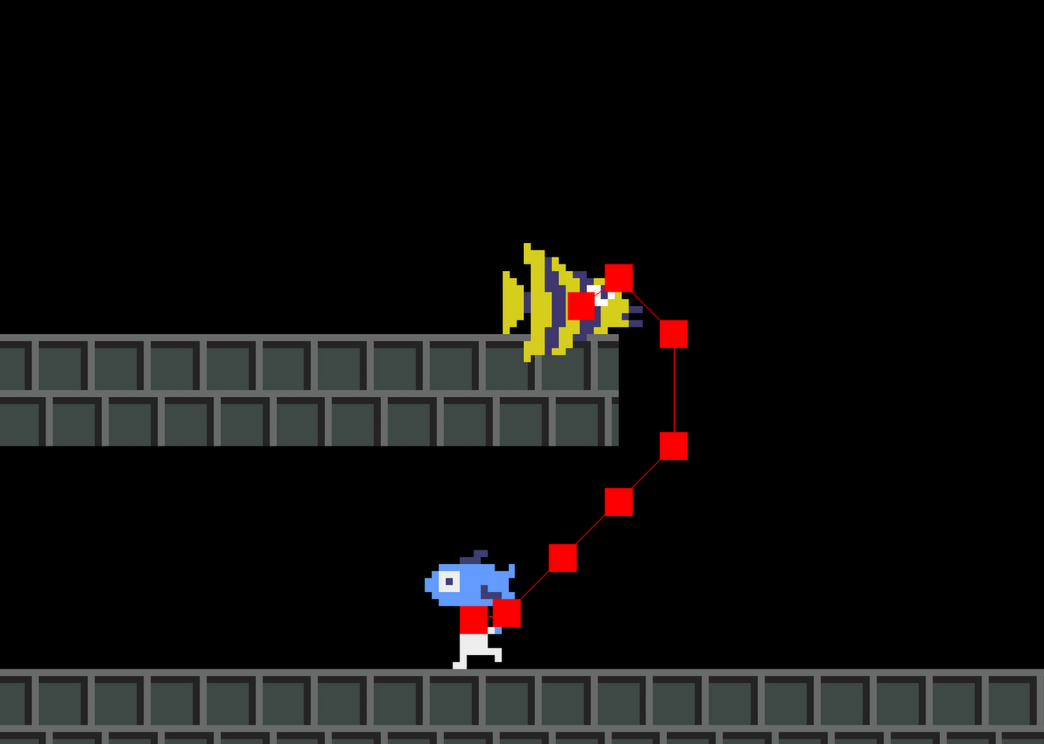
\includegraphics[scale=0.35]{img/triangle-chase-2.png}
    \caption[Ejemplo del pathfinding del enemigo Triangle Fish]{Ejemplo del pathfinding del enemigo Triangle Fish.}
    \label{fig:triangle-chase-2}
\end{figure}

Con el objetivo de lograr una jugabilidad más divertida, el enemigo solo genera un camino cuando pierde de vista al jugador, es decir, cuando hay algún obstáculo entre ellos. En caso contrario, se sigue una estrategia más simple y menos eficiente: primero se desciende hasta alcanzar la altura del jugador, y luego se avanza en linea recta, como se muestra en la figura \ref{fig:triangle-chase-1}. Esto permite al jugador evadir al enemigo saltándolo, cosa que sería imposible si este siempre siguiera el camino óptimo. 

\begin{figure}[h]
    \centering
    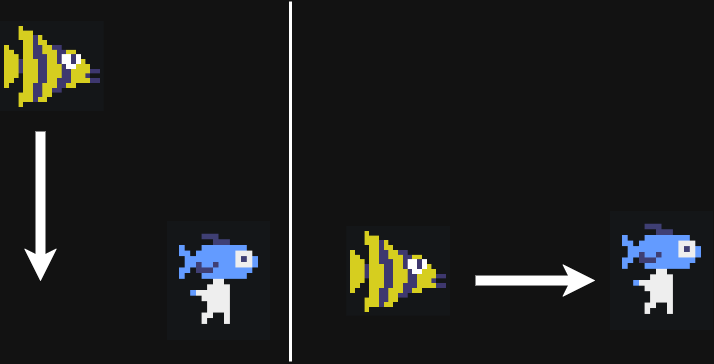
\includegraphics[scale=0.45]{img/triangle-chase-1.drawio.png}
    \caption[Esquema de estrategia de persecución de Triangle Fish]{Esquema de estrategia de persecución de Triangle Fish. Primero desciende hasta la altura del jugador y luego avanza en línea recta.}
    \label{fig:triangle-chase-1}
\end{figure}

%% FALTA EXPLICAR LAS OLEADAS

\section{Otros sistemas}

En este apartado se describirán otras implementaciones y funcionalidades del proyecto.

\subsection{Funciones de guardado}

El juego cuenta con tres espacios (\textit{slots}) para que el jugador guarde partida. Es decir, se puede guardar el progreso de tres partidas distintas de forma simultánea. La funcionalidad de guardado está encapsulada en el autoload \textit{DataManager}. Este expone funciones que otras escenas usan para solicitar guardar o cargar el progreso de la partida. Por ejemplo, en la escena \textit{SelectFile} el usuario elige uno de los tres slots para cargar partida. Esta escena recoge los datos de todas las partidas guardadas para exponerlas en forma de menú.

Para almacenar de forma persistente los datos de guardado se utilizaron los \textbf{recursos} de Godot. Mientras que los nodos son unidades de funcionalidad, los recursos son contenedores de datos. Pueden ser asignados como el tipo de una variable en una escena. Además, Godot cuenta con funciones para guardarlos fácilmente en el disco. Cuando se carga un recurso, el motor guarda una única copia del mismo en memoria. Eso quiere decir que si se modifica y otra escena lo carga posteriormente, tendrá acceso a la versión modificada del mismo.

Algunos nodos en Godot cuentan con recursos por defecto como Sprite2D, que contiene un nodo Texture2D para añadir una imagen. Sin embargo se pueden definir recursos personalizados. En este caso, se definieron los recursos \textbf{SaveData} para almacenar el progreso de la partida y \textbf{PlayerData} para el estado actual del jugador. En la figura \ref{fig:save-diagram} se muestra un diagrama de clases para \textit{DataManager} y sus recursos.

\begin{figure}[h]
    \centering
    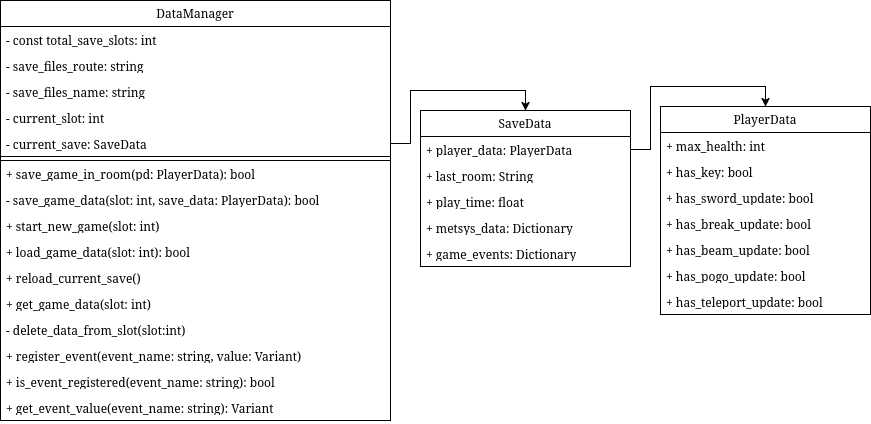
\includegraphics[scale=0.45]{img/save-data-diagram.drawio.png}
    \caption[Diagrama de clases de funciones de guardado]{Diagrama de clases de funciones de guardado. SaveManager hace de interfaz para que otras escenas accedan a los datos de guardado.}
    \label{fig:save-diagram}
\end{figure}

Los datos de progreso usados internamente por el plugin MetSys (mapa explorado, objetos coleccionados, etc.) están en formato de diccionario y cuenta con funciones para cargarlos, por lo que se guardan fácilmente en \textit{SaveData}. Se añadió también un diccionario adicional para guardar ciertos eventos. Por ejemplo, si una horda de enemigos ya ha sido derrotada en una sala, se almacena esa información para no instanciar la misma horda la próxima vez que el jugador visite la sala.

\subsection{Asignación de controles}

Godot cuenta con un mapa de controles para el jugador. En este se pueden definir acciones como podrían ser \textit{jump}, \textit{atack} o \textit{move\_left} y asignarlas a un botón de un mando o teclado. Sin embargo, esta asignación es estática. El jugador requiere por accesibilidad la opción de poder modificar el esquema de controles en su teclado o mando.

Para implementar esta funcionalidad se incluyó el plugin \textbf{Godot Controls Remap (GCR)}\cite{controls-remap}. Este permite reasignar de forma dinámica las acciones de Godot a cualquier otro input. Para operarlo se implementó el autoload \textbf{InputMapper}, que hace de interfaz para la reasignación de controles. Se encarga de cargar y guardar en memoria el esquema actual de controles y de captar inputs del usuario para asignarlos a la acción correspondiente. Una vez hecha la reasignación, el resto de escenas que capten la entrada del usuario podrán hacerlo de forma normal, con la función \textit{\_input(event)} o el singleton \textit{Input}.

Para comunicar los controles del juego, es necesario mostrar para cada acción el icono de su tecla o botón asociado. Como estos pueden reasignarse, este icono no puede ser estático. Para solventar esto se usó \textbf{Godot Action Icon}\cite{action-icon}. Este plugin permite definir un mapa acción-icono para mostrar en pantalla. Además, actualiza el esquema de iconos entre teclado y mando en función de cual esté usando el usuario actualmente. Incluye también un pack de iconos por defecto de uso libre\cite{icon-pack}.

\subsection{Traducción}

Todos los textos del juego están disponibles tanto en inglés como en español. El usuario puede seleccionar le idioma en el menú de opciones. Para gestionar el cambio de idioma se implementó el autoload \textbf{LocalizationManager}. Este define los idiomas en los que está disponible el juego y aplica los cambios a través de \textit{TranslationServer}, el autoload de Godot responsable gestionar las traducciones. 

Se creó una hoja de cálculo con el formato que se muestra en la tabla \ref{tab:localization-table}. Para cada texto se tiene una etiqueta y una traducción en inglés y español. En los elementos del juego en lugar de ecribir los textos finales, se escriben sus etiquetas. Una vez se define un código de idioma como activo en el TranslationServer, todas las etiquetas del juego son sustituidos por la traducción en tiempo de ejecución.

\begin{table}[!ht]
    \centering
    \begin{tabular}{|l|l|l|}
    \hline
        keys & en & es \\ \hline
        NEWGAME & New game & Nueva partida \\ \hline
        CONTINUE & Continue & Continuar \\ \hline
        SETTINGS & Settings & Ajustes \\ \hline
        EXIT & Exit & Salir \\ \hline
        RESUME & Resume & Continuar \\ \hline
        BACK & Back & Volver \\ \hline
        EXIT & Exit & Salir \\ \hline
        LANGUAGE & Language & Idioma \\ \hline
    \end{tabular}
    \caption{Ejemplo de la tabla de traducciones.}
    \label{tab:localization-table}
\end{table}

\subsection{Reloj}

En la pantalla final del juego, cuando el jugador lo completa, se muestra el tiempo que este ha tardado en hacerlo. Este tiempo cuenta únicamente los momentos en los que el jugador se encuentra en el mundo, no cuando se pausa el juego, por ejemplo. Para gestionar este conteo, se hizo el autoload \textbf{Clock}. Este lleva una sumatoria del tiempo transcurrido, la cual se guarda junto al resto de datos de la partida. Se conecta a una colección de señales de \textit{GameEvent} y estas, al emitirse, llaman a funciones de \textit{Clock} que inician, pausan o reinician el conteo de tiempo.

De esta manera, si un nodo emite la señal de \textit{GameEvent} para pausar el juego, \textit{Clock} la recibe y detiene el cronómetro. La escena que emitió la pausa sin embargo no es consciente del reloj, reduciendo el acoplamiento de la funcionalidad.

\subsection{Diálogos}

Para implementar los diálogos se incluyó en el proyecto el plugin \textbf{Godot Dialogue Manager}. Entre sus funcionalidades destacan:

\begin{itemize}
    \item Instanciación de burbujas de diálogo con aspecto personalizable.
    \item Scripting de diálogos potente con opción a ramificaciones, condicionales y lectura de variables entre otros.
    \item Soporte para traducciones.
    \item Reproducción de voces.
\end{itemize}

Los diálogos se instancian a través del autoload del plugin, \textit{DialogueManager}. Para ello se necesitan dos elementos:

\begin{itemize}
    \item Un \textit{script} que contenga todo el texto del diálogo. Esto se almacena en un archivo con extensión .dialogue.
    \item Una escena que contenga los elementos visuales del diálgo como el marco o la tipografía. Para este proyecto se usa la escena \textit{Balloon}.
\end{itemize}

Los diálogos siempre son emitidos por un NPC (personaje no jugable) cuando el jugador interactua con este. Se creó el componente \textit{DialogueComponent} (ver figura \ref{fig:dialogue-component}), que está incluido por defecto en todas las escenas \textit{NpcCharacter}. Este hereda de un \textit{Area2D}. Cuando este área detecta que el jugador ha entrado en el rango en el que puede interactuar con el NPC, se muestra una flecha para indicárselo. Cuando recibe el \textit{input} del jugador, se arranca el flujo de interacción que instanciará el diálogo, el cual se muestra en la figura \ref{fig:dialogue-flow}.

\begin{figure}[h]
    \centering
    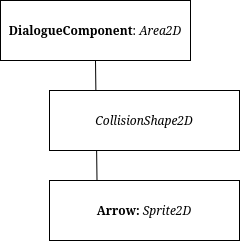
\includegraphics[scale=0.45]{img/dialogue-component.drawio.png}
    \caption[Arquitectura de la escena DialogueComponent]{Arquitectura de la escena DialogueComponent.}
    \label{fig:dialogue-component}
\end{figure}

\begin{figure}[h]
    \centering
    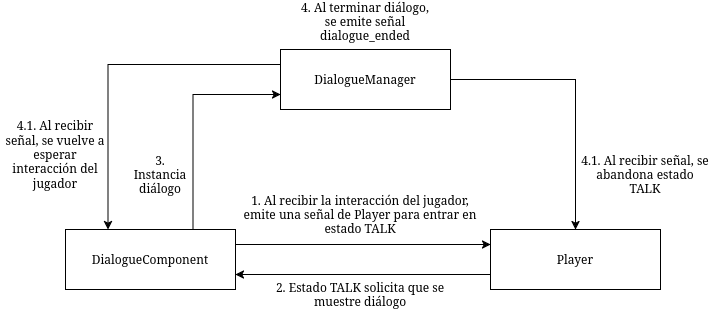
\includegraphics[scale=0.55]{img/dialogue-flow.drawio.png}
    \caption[Flujo de interacciones para iniciar y finalizar un diálogo.]{Flujo de interacciones para iniciar y finalizar un diálogo desde una interacción del jugador.}
    \label{fig:dialogue-flow}
\end{figure}

\subsection{Implementación de máquina de estados}
\label{sec:state-machine}

La implementación del patrón de máquina de estados de este proyecto está basado en el propuesto por GDQuest\cite{fsm-gdquest}. En la figura \ref{fig:state-machine-diagram} se tiene un diagrama de clases. Cuando una escena necesita de una máquina de estados se le añade un nodo \textbf{StateMachine}. Este tiene como hijos tantos nodos \textbf{State} como estados existan, los cuales contienen el código asociado a su lógica. StateMachine se encarga de realizar las transiciones entre estados.

Cuando un estado entra en activo, ejecuta su código de iniciación (\textit{\_enter()}). Al darse la condición para que transicione, emite la señal \textit{finished}. StateMachine la recibe y se encarga de ejecutar su código de finalización (\textit{\_exit()}) y transicionar al siguiente estado.

\textit{State} es una interfaz. Para cada máquina de estados es necesario crear una clase que herede de esta, como se ve en la figura \ref{fig:state-machine-diagram}. En el caso del jugador, se tiene la clase \textit{PlayerState}, que guarda una referencia a \textit{Player} y define en constantes todos los estados posibles para esta máquina. Posteriormente, se crea un script para cada estado que herede de este (\textit{idle.gd, move.gd, jump.gd, etc}).

\begin{figure}[h]
    \centering
    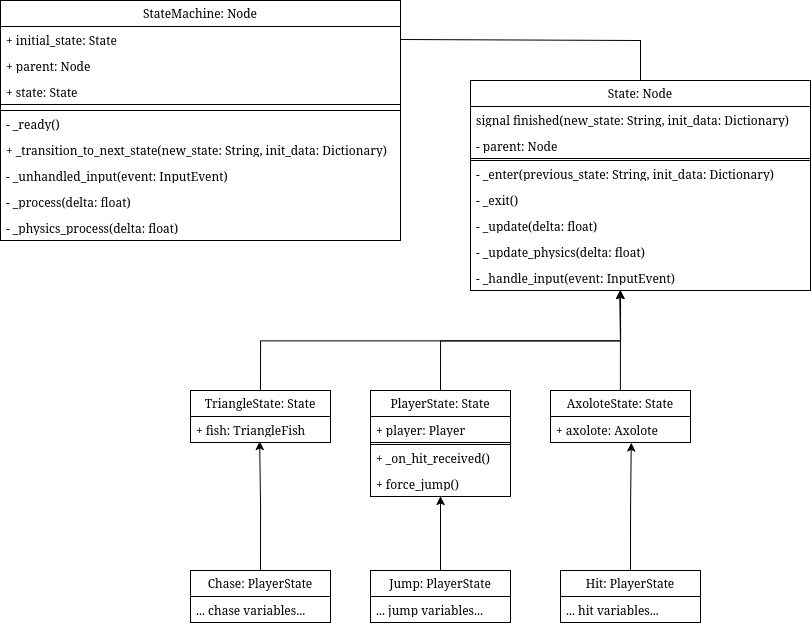
\includegraphics[scale=0.45]{img/state-machine.drawio.png}
    \caption[Diagrama de clases para la implementación de la máquina de estados.]{Diagrama de clases para la implementación de la máquina de estados.}
    \label{fig:state-machine-diagram}
\end{figure}

Normalmente, es la lógica interna del estado la que define cuando es momento de transicionar a otro. Es posible que esta transición necesite responder a un evento externo, como ocurre con \textit{HIT}, que se inicia al ser golpeado. Para no tener que implementar la lógica de detección de golpes en todos los estados de Player, se puede añadir una puerta de entrada en PlayerState para este tipo de eventos, como \textit{\_on\_hit\_received().}

Por último, es posible que un estado necesite de ciertos datos para su funcionamiento. Cuando un enemigo es golpeado, sale disparado en una dirección. El estado \textit{HIT} necesita esa dirección. Es por esto que la función \textit{\_enter()} cuenta con un parámetro de tipo diccionario, donde se le pueden pasar los parámetros que necesite.

\section{Interfaz de usuario}

% cómo están hechos los menús (nodos control)

Los menús del juego tales como la pantalla de título o de ajustes están hechos con \textbf{nodos de control}. Estos son una colección de nodos nativos de Godot diseñados para construir interfaces de usuario. Cuentan con utilidades para crear botones, \textit{sliders}, \textit{checkbox} y centrar elementos entre otras. Tiene soporte por defecto para interacción con mando, teclado o ratón.

Como se muestra en la figura \ref{fig:controls-menu}, la interfaz se contruye añadiendo nodos de forma jerárquica para cada uno de los elementos. Cada pantalla de menú es una escena. Un script asociado a la raíz de la escena contiene su lógica y dota de funcionalidad a todos los botones y demás elementos interactuables.

\begin{figure}[h]
    \centering
    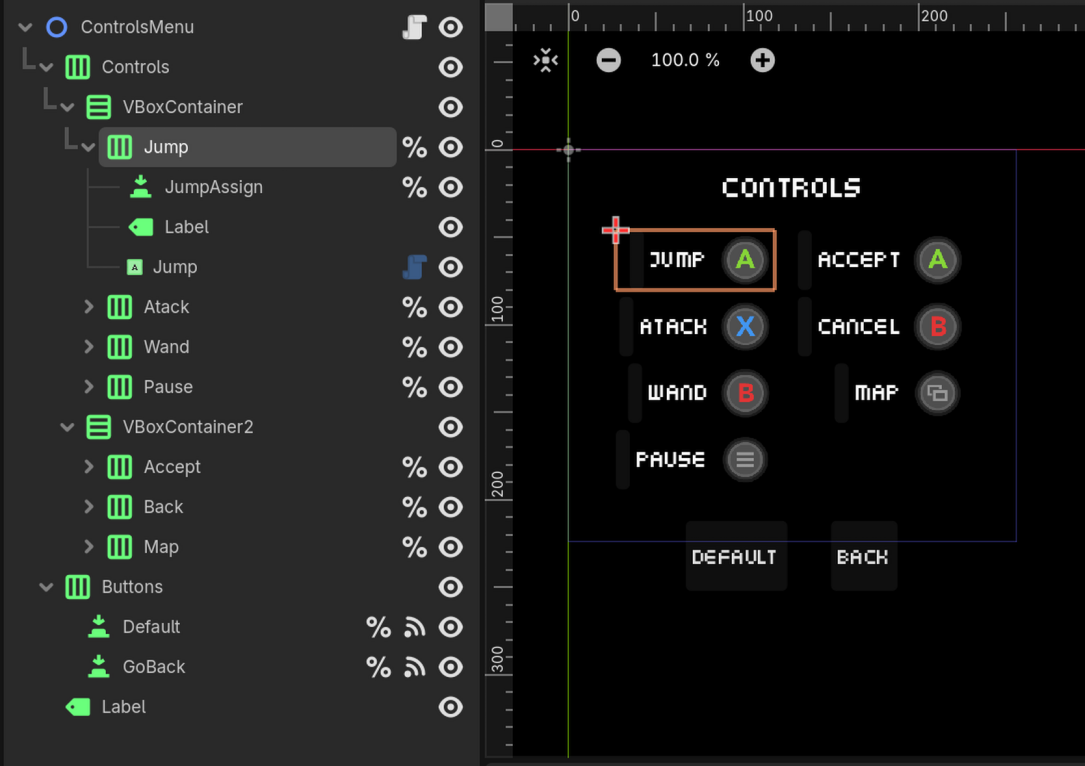
\includegraphics[scale=0.35]{img/controls-menu.png}
    \caption[Captura de pantalla de la estructura del menú de controles.]{Captura de pantalla de la estructura del menú de controles.}
    \label{fig:controls-menu}
\end{figure}

% comentar la aplicación de tema

El aspecto de todos los elementos de tipo control puede ser modificado. Esto incluye su color, tamaño, borde, tipografía, etc. Ajustar esto para cada elemento sería muy costoso, por lo que se hace uso de los \textbf{temas} de Godot. Estos son recursos usados para estilizar nodos de tipo \textit{window} o control. Pueden definir el aspecto para todos los elementos de la interfaz. Los temas se establecen en el nodo raíz de la escena y sus nodos hijos lo heredan. Es posible también establecer un tema como predeterminado, de tal forma que se asignen a todos los nodos control al crearlos.

% mencionar que los menús de mapa son componentes importados de metsys

En apartados anteriores se comentó que los menús de mapa y mini-mapa son componentes importados del plugin MetSys, por lo que no hay mucho que comentar sobre ellos. Estos renderizan una vista que permanece estática en la pantalla, por lo que ambos se dispusieron sobre un nodo \textit{CanvasLayer}. Este permite la renderización independiente de objetos 2D en una escena. Esto quiere decir que las coordenadas heredadas del nodo padre serán ignoradas y el posicionamiento será, a efectos prácticos, relativo al \textit{viewport} del juego.

% playerui, interacción con player y game event

El resto de la interfaz consiste en un marco que rodea toda la pantalla y contiene los puntos de salud totales y restantes del jugador. Estos se renderizan a través de la escena \textit{PlayerUi}. La escena escucha una señal del autoload \textit{GameEvent} que se emite desde la escena Player cuando el jugador gana o pierde salud, o cuando obtiene un objeto para aumentar su vida máxima. Una vez se recibe la señal, se actualiza el estado y se renderiza en pantalla los elementos correspondientes. En la figura \ref{fig:ui-hearts} se tiene una captura de pantalla de esta interfaz.

\begin{figure}[h]
    \centering
    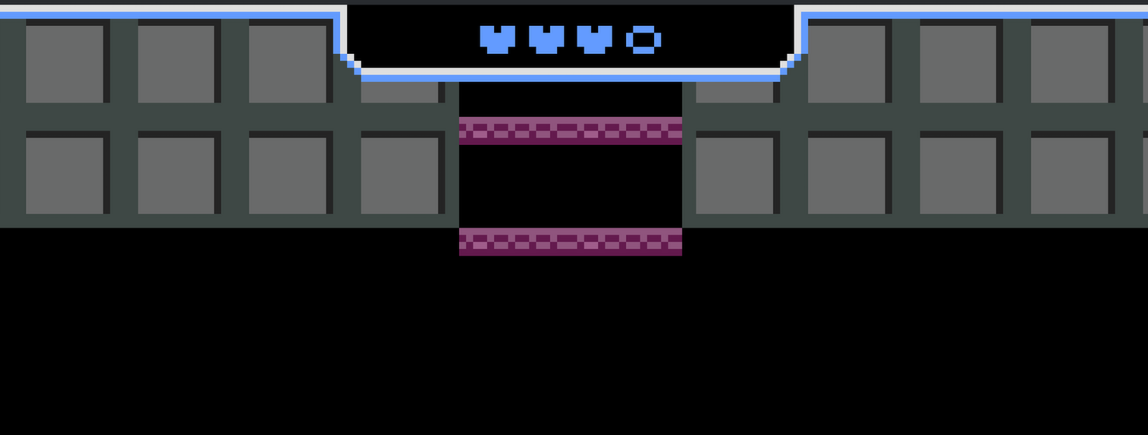
\includegraphics[scale=0.35]{img/ui-hearts.png}
    \caption[Captura de pantalla de la interfaz de salud del jugador.]{Captura de pantalla de la interfaz de salud del jugador. Se tienen 4 corazones como máximo. El jugador ha sido golpeado, por lo que solo le quedan otros 3.}
    \label{fig:ui-hearts}
\end{figure}

\section{Accesibilidad y ajustes}

% Mencionar la implementación de los ajustes, diagramas de clase para los parámetros

En el menú de ajustes, el jugador tiene una serie de opciones para configurar su experiencia:

\begin{itemize}
    \item Selección de idioma.
    \item Selección de volumen en tres canales: se puede regualr el volumen general o de música y sonido por separado. Esto se hizo configurando en el proyecto 3 buses de audio (\textit{master}, \textit{music} y \textit{SFX}). Cada nodo de audio del juego está asociado al bus \textit{music} o \textit{SFX}. Desde el menú de ajuste se baja el volumen asociado a estos buses o al general.
    \item Entrar o salir de pantalla completa.
    \item Ajuste de brillo y contraste de la pantalla. Este efecto se implementó utilizando los \textit{WorldEnvironment} de Godot, usados para el postprocesado de escenas.
    \item Reasignación de controles.
\end{itemize}

El jugador accede a estas opciones desde la escena \textit{SettingsMenu}. Esta opera la interfaz del autoload \textit{SettingsManager} para aplicar las configuracones. Es este último también el encargado de guardarlas en memoria usando el recurso customizado \textit{SettingsData}. En la figura \ref{fig:settings-diagram} se tiene un diagrama de este planteamiento.

\begin{figure}[h]
    \centering
    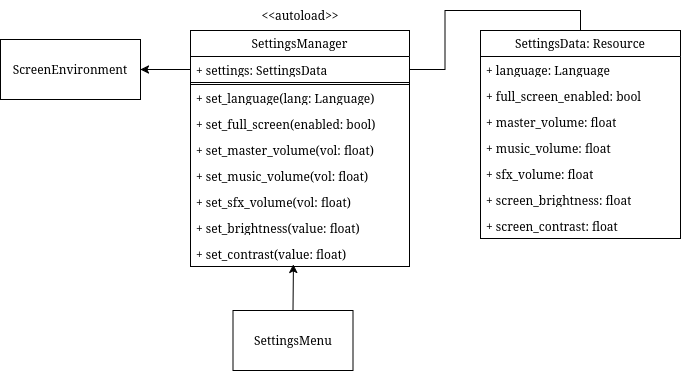
\includegraphics[scale=0.55]{img/setteings.drawio.png}
    \caption[Diagrama de clases y escenas para los ajustes del juego.]{Diagrama de clases y escenas para los ajustes del juego.}
    \label{fig:settings-diagram}
\end{figure}

%% ACCESIBILIDAD
A continuación se repasarán las consideraciones que se tuvieron respecto a la accesibilidad y su relación con los ajustes previamente explicados si la tuvieran.

% auditiva
% todos los textos del juego son más grandes que el mínimo de píxeles recomendado, con fondo negro. El usuario puede ajustar el volumen de los 3 canales. No hay ningún elemento que requiera de sonido para avanzar

En cuanto a \textbf{accesibilidad auditiva y visual}, todos los textos del juego son más grandes que el tamaño mínimo de fuente recomendado (46 píxeles). Aparecen siempre sobre un fondo negro y es el usuario el que avanza el texto a voluntad. El juego no tiene voces, por lo que el texto es el único canal de comunicación en ese sentido. El usuario puede regular el volumen diferenciando entre general, música y sonido. Tampoco existe ningún elemento de juego que requiera de escuchar audio para poder progresar.

% visual/daltonismo
% mencionar colores del mapeado

Para garantizar la \textbf{accesibilidad de las personas con daltonismo} se usó la herramienta ColorBlindnessTest\cite{simulador-daltonismo}. Esta permite a partir de una imagen simular cómo la verían usuarios con ciertos tipos de daltonismo. Esto es especialmente útil para detectar si los distintos colores se diferenciarían bien. El mapa del juego se divide en tres zonas principales. Cada una de estas zonas tiene motivos de color distintos. Esto ayuda a orientarse y recordar salas más fácilmente. Para asegurar que estas zonas serían diferenciadas sin problema, se cargó en la herramienta el \textit{tile atlas} del mapa. Finalmente se eligieron los colores gris, naranja y azul para las tres zonas principales. Como se puede ver en la figura \ref{fig:daltonismo-comparacion}, las tres últimas filas de color son diferenciadas en todos los principales tipos de daltonismo.

\begin{figure}[h]
    \centering

    \begin{minipage}{0.45\textwidth}
        \centering
        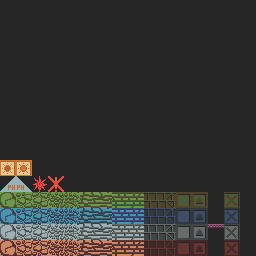
\includegraphics[width=\linewidth]{img/tritanomalía.png}
    \end{minipage}
    \hfill
    \begin{minipage}{0.45\textwidth}
        \centering
        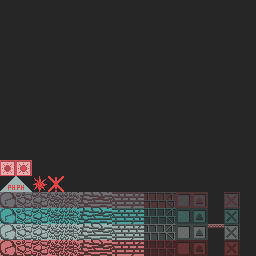
\includegraphics[width=\linewidth]{img/tritanopia.png}
    \end{minipage}

    \vspace{0.3cm}

    \begin{minipage}{0.45\textwidth}
        \centering
        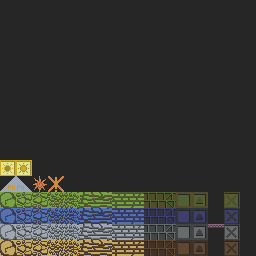
\includegraphics[width=\linewidth]{img/protanomaly.png}
    \end{minipage}
    \hfill
    \begin{minipage}{0.45\textwidth}
        \centering
        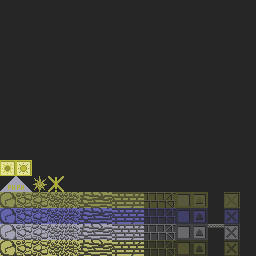
\includegraphics[width=\linewidth]{img/protanopia.png}
    \end{minipage}

    \caption{Simulación de diferentes tipos de daltonismo para el tileset del juego. Los colores originales de las filas corresponden a verde, azul, gris y naranja respectivamente.}
    \label{fig:daltonismo-comparacion}
\end{figure}

% motora
% reasignación de controles, compatible con cualquier entrada

Para la \textbf{accesibilidad motora} se cuenta con la ya expuesta reasignación de controles. Esta es compatible para cualquier entrada tanto de teclado como de mando, por lo que incluso usuarios con mandos especializados para su diversidad funcional motora podrán jugar. El juego además tiene un ritmo lento en su jugabilidad. No es exigente ni difícil en lo que al control se refiere y se centra más en la exploración, lo cual supone un impedimento menos para usuarios de este perfil.

% cognitiva
% analisis de sobrecarga sensorial
% mencionar ajuste de brillo y contraste

En cuanto a \textbf{accesibilidad cognitiva}, se realizó un análisis de un segmento del juego utilizando la herramienta \textit{Video Flash Analysis}\cite{video-flash-analysis} para asegurar que cumple los estándares para la protección de usuario con epilepsia fotosensible y otras sensibilidades. El resultado del análisis fue positivo como se muestra en al figura \ref{fig:settings-diagram}. Además, el usuario puede modificar el brillo y el contraste por si siente alguna molestia.

\begin{figure}[h]
    \centering
    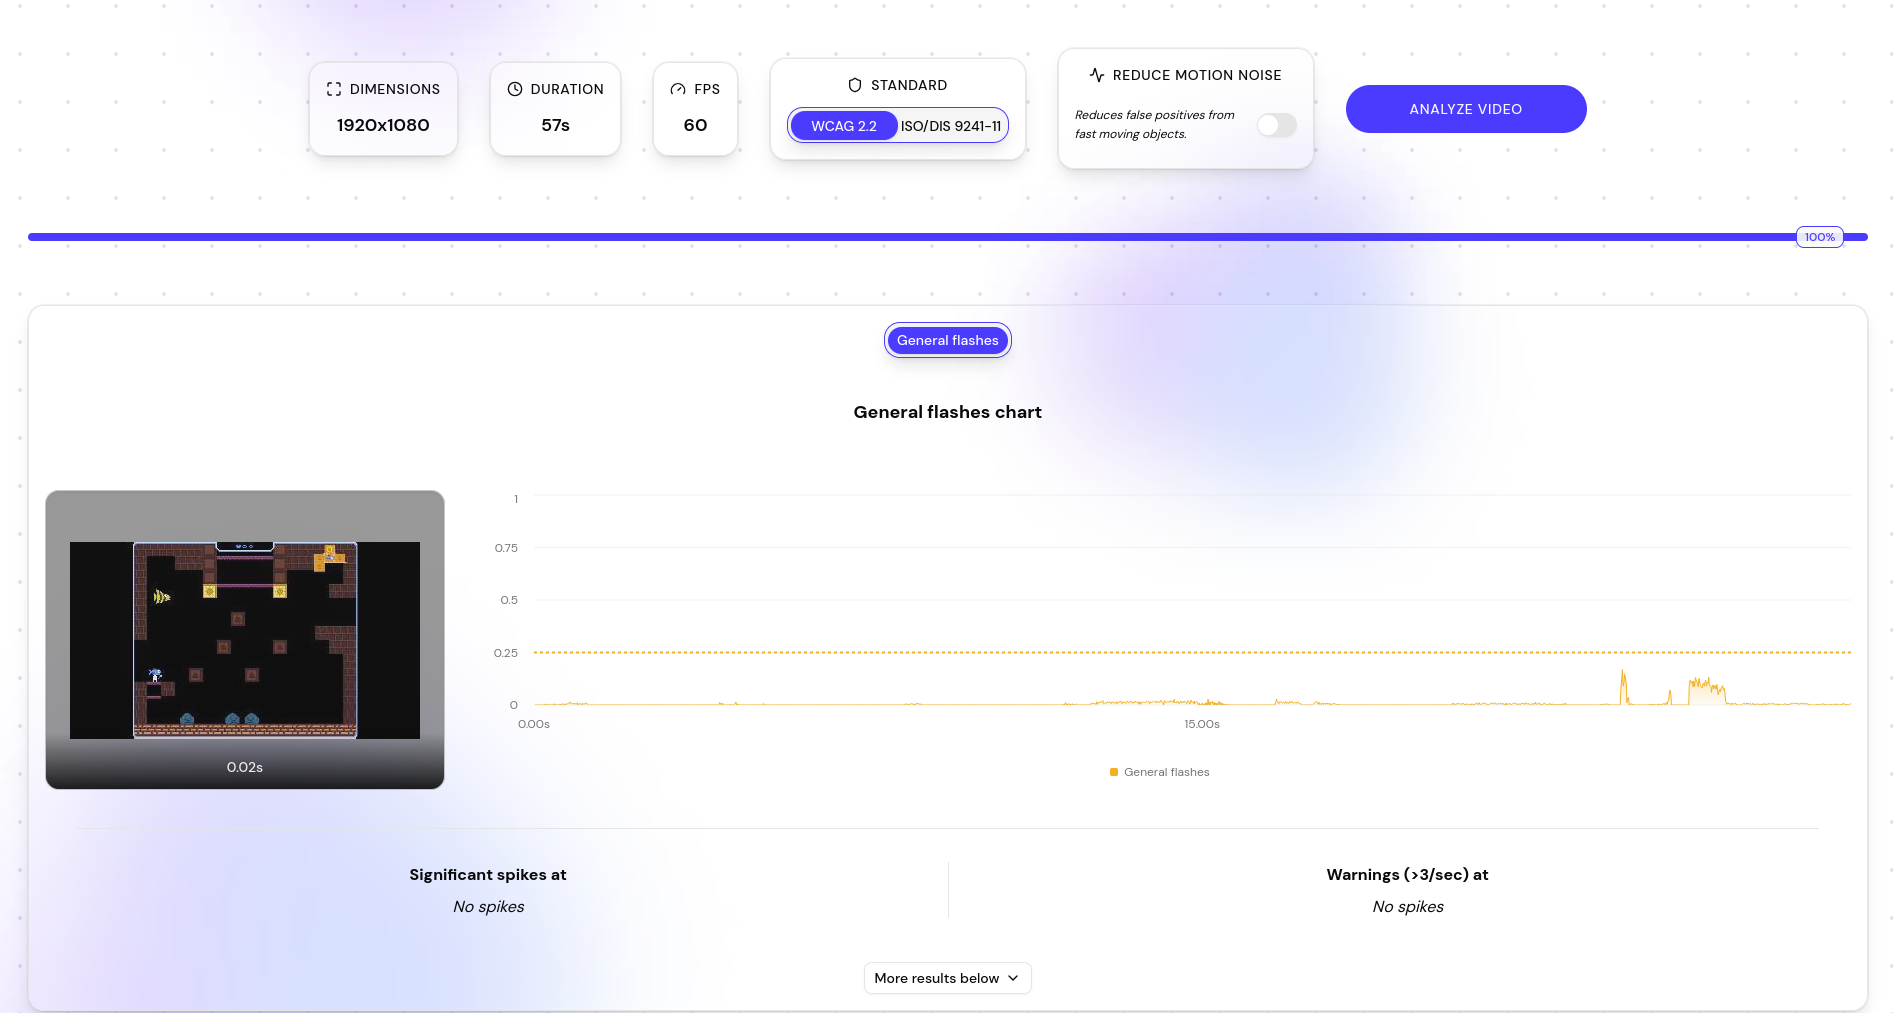
\includegraphics[scale=0.30]{img/test-fotosensible.png}
    \caption[Resultado de análisis de fotosensibilidad para un fragmento de video del juego.]{Resultado de análisis de fotosensibilidad para un fragmento de video del juego.}
    \label{fig:settings-diagram}
\end{figure}

% 

\section{CI/CD/Testing}

% hablar de gdunit

Para desarrollar los tests automáticos del proyecto se usó \textit{GDUnit4}\cite{gdunit4}, un framework embebido en Godot que permite el desarrollo de tests unitarios y de integración. También permite detectar filtraciones de memoria, monitorizar el rendimiento y detectar escenas huérfanas en el árbol de escena. Se priorizó el desarrollo de tests para las funciones centrales y estructurales del proyecto, dejando de lado otros sistemas más tangentes que posiblemente cambiarían a lo largo del desarrollo. En la figura \ref{fig:gdunit-execution} se tiene un ejemplo de ejecución de los tests del proyecto. En la tabla \ref{tab:test-table} se tiene el listado de tests del proyecto.

\begin{figure}[h]
    \centering
    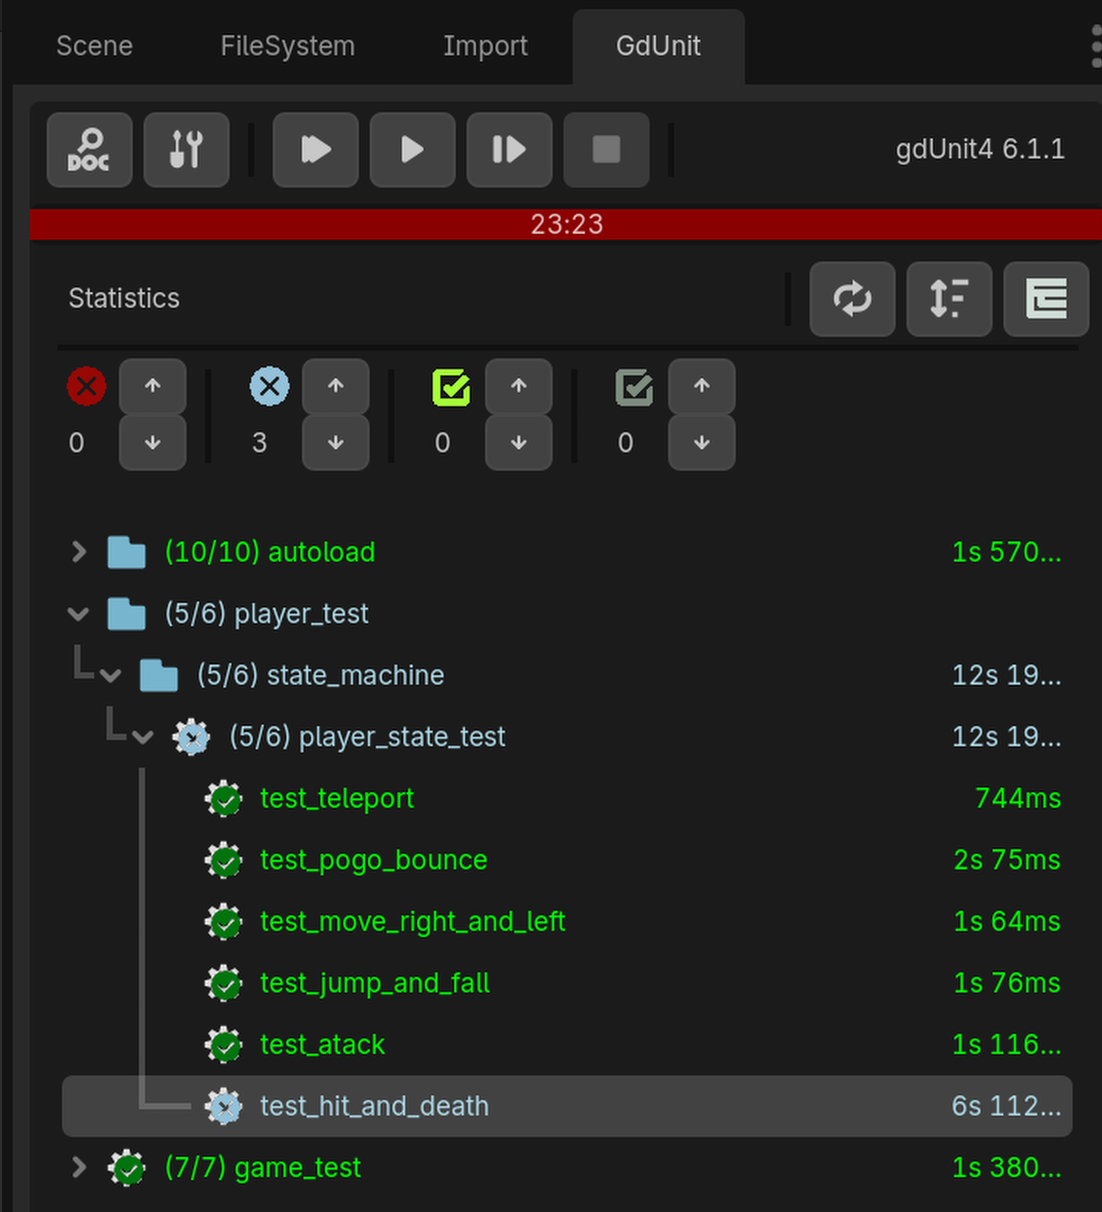
\includegraphics[scale=0.30]{img/gdunit.png}
    \caption[Captura de pantalla de interfaz de gdUnit4 embebida en godot.]{Resultado de ejecución de tests del proyecto en la interfaz de gdUnit4. Como se puede observar, un test de Player ha fallado.}
    \label{fig:gdunit-execution}
\end{figure}

% poner tabla con tests

\begin{table}[!ht]
    \centering
    \begin{tabular}{|p{4cm}|p{6cm}|p{2cm}|}
    \hline
        Nombre de test & Descripción & Módulo \\ \hline
        test teleport & Verifica que el jugador entra en estados de teletransporte y cambia posición correctamente & Player \\ \hline
        test pogo bounce & Comprueba que el ataque hacia abajo en el aire activa el estado POGO y rebote vertical & Player \\ \hline
        test move right and left & Valida el movimiento horizontal del jugador hacia derecha e izquierda y estados asociados & Player \\ \hline
        test jump and fall & Comprueba que el jugador puede saltar y entra en estado de salto sin estar en el suelo & Player \\ \hline
        test atack & Verifica que el ataque activa el estado ATACK y detiene el movimiento horizontal & Player \\ \hline
        test hit and death & Comprueba el sistema de daño, invencibilidad temporal y transición a estado DEAD & Player \\ \hline
        test remap action key & Verifica que las acciones pueden remapearse correctamente y responden a la nueva tecla asignada & InputManager \\ \hline
        test starting state & Comprueba que el juego inicia en el estado de pantalla de título & Game \\ \hline
        test start new game & Verifica la transición desde título a intro y luego a GameWorld & Game \\ \hline
        test load game and pause game & Comprueba que el juego puede pausarse y reanudarse correctamente desde el GameWorld & Game \\ \hline
        test return to title screen & Verifica que se puede volver a la pantalla de título desde el menú de pausa & Game \\ \hline
        test load game die and respawn & Comprueba la transición a GAME\_OVER y la correcta reaparición en el mundo de juego & Game \\ \hline
        test load game finish game and return to title & Verifica el flujo de final del juego y retorno a la pantalla de título & Game \\ \hline
        test forbidden game state changes & Comprueba que transiciones de estado no permitidas son ignoradas correctamente & Game \\ \hline
    \end{tabular}
    \caption{Tabla de tests automáticos del proyecto.}
    \label{tab:test-table}
\end{table}

% hablar de github action para ejecución de tests en remoto

Para asegurar que los cambios producidos durante el desarrollo no rompían ninguna funcionalidad previa, se configuró en el repositorio de Github una Github Action (GdUnit4 Test\cite{gdunit4-action}) que se ejecuta cada vez que se pushea algún commit a remoto. Esta crea una máquina virtual y ejecuta todos los test del proyecto. Si algún test falla, se notifica al usuario a través de correo electrónico. Esta comprobación se realiza también antes de cerrar un pull request, impidiendo que alguna rama con fallos se mezcle en otra. Para configurar esta acción se añadió el siguiente script .yaml a la carpeta \textit{.github/workflows}:

\begin{verbatim}
name: GdUnit4 Tests (wip)
on: [push, pull_request]

jobs:
  test:
    runs-on: ubuntu-latest
    permissions:
      contents: read
      checks: write
    steps:
      - uses: actions/checkout@v4
      - uses: godot-gdunit-labs/gdUnit4-action@v1
        with:
          godot-version: '4.6'
          project_dir: './game/'
          paths: 'res://test'
\end{verbatim}

Se configuró otra \textit{Github Action} para desplegar automáticamente el juego en \textit{Itch.io} con compilaciones para las plataformas Windows, Linux y Web. El script para describir la acción se basó en el propuesto por Nepo\cite{nepo-ci}, el cual usa la imagen de Docker \textit{godot-ci}\cite{godot-ci}. Para desplegar el proyecto se empleó \textit{butler}\cite{butler}. El script resultante es el siguiente:

\begin{verbatim}
name: Build + Deploy
on:
  push:
    branches:
      - 'release/**'
      - 'playtest/**'

  pull_request:
    branches:
      - 'release/**'
      - 'playtest/**'

  workflow_dispatch:

env:
  ITCHIO_USERNAME: pavro-o
  ITCHIO_GAME: mero-mero
  BUTLER_API_KEY: ${{ secrets.BUTLER_API_KEY }}
  GODOT_VERSION: 4.6.2
  PROJECT_FOLDER: game

jobs:
  web:
    name: Build and deploy to itch.io
    runs-on: ubuntu-latest
    container:
      image: barichello/godot-ci:4.6.2
    steps:
      - name: Checkout
        uses: actions/checkout@v2
        with:
          lfs: true
      - name: Setup
        run: |
          mkdir -v -p ~/.local/share/godot/export_templates
          mv /root/.local/share/godot/export_templates/${GODOT_VERSION}.stable ~/.local/share/godot/export_templates/${GODOT_VERSION}.stable
      
      # If you don't want to do a web build, remove the following section
      - name: Web Build
        run: |
          cd ${PROJECT_FOLDER}
          mkdir -p build/web
          godot --export-release --headless "Web" ./build/web/index.html
      
      - name: Windows Build
        run: |
          cd ${PROJECT_FOLDER}
          mkdir -p build/windows
          godot --export-release --headless "Windows" ./build/windows/game.exe

      - name: Linux Build
        run: |
          cd ${PROJECT_FOLDER}
          mkdir -p build/linux
          godot --export-release --headless "Linux" ./build/linux/game.x86_64
      - name: Itch.io Deploy

        run: |
          ls ./${PROJECT_FOLDER}/build
          butler push ./${PROJECT_FOLDER}/build/web $ITCHIO_USERNAME/$ITCHIO_GAME:html5
          butler push ./${PROJECT_FOLDER}/build/windows $ITCHIO_USERNAME/$ITCHIO_GAME:windows
          butler push ./${PROJECT_FOLDER}/build/linux $ITCHIO_USERNAME/$ITCHIO_GAME:linux
\end{verbatim}